%  LaTeX support: latex@mdpi.com 
%  For support, please attach all files needed for compiling as well as the log file, and specify your operating system, LaTeX version, and LaTeX editor.

%=================================================================
\documentclass[bdcc,article,submit,moreauthors]{Definitions/mdpi}
%\documentclass[preprints,article,submit,moreauthors]{Definitions/mdpi} 
% For posting an early version of this manuscript as a preprint, you may use "preprints" as the journal. Changing "submit" to "accept" before posting will remove line numbers.

% Below journals will use APA reference format:
% admsci, aieduc, behavsci, businesses, econometrics, economies, education, ejihpe, famsci, games, humans, ijcs, ijfs, jintelligence, journalmedia, jrfm, jsam, languages, peacestud, psycholint, publications, tourismhosp, youth

% Below journals will use Chicago reference format:
% arts, genealogy, histories, humanities, laws, literature, religions, risks, socsci

%--------------------
% Class Options:
%--------------------
%----------
% journal
%----------
% Choose between the following MDPI journals:
% accountaudit, acoustics, actuators, addictions, adhesives, admsci, adolescents, aerobiology, aerospace, agriculture, agriengineering, agrochemicals, agronomy, ai, aichem, aieduc, aieng, aimater, aimed, aipa, air, aisens, algorithms, allergies, alloys, amh, analog, analytica, analytics, anatomia, anesthres, animals, antibiotics, antibodies, antioxidants, applbiosci, appliedchem, appliedmath, appliedphys, applmech, applmicrobiol, applnano, applsci, aquacj, architecture, arm, arthropoda, arts, asc, asi, astronautics, astronomy, atmosphere, atoms, audiolres, automation, axioms, bacteria, batteries, bdcc, behavsci, beverages, biochem, bioengineering, biologics, biology, biomass, biomechanics, biomed, biomedicines, biomedinformatics, biomimetics, biomolecules, biophysica, bioresourbioprod, biosensors, biosphere, biotech, birds, blockchains, bloods, blsf, brainsci, breath, buildings, businesses, cancers, carbon, cardio, cardiogenetics, cardiovascmed, catalysts, cells, ceramics, challenges, chemengineering, chemistry, chemosensors, chemproc, children, chips, cimb, civileng, cleantechnol, climate, clinbioenerg, clinpract, clockssleep, cmd, cmtr, coasts, coatings, colloids, colorants, commodities, complexities, complications, compounds, computation, computers, condensedmatter, conservation, constrmater, cosmetics, covid, crops, cryo, cryptography, crystals, csmf, ctn, culture, curroncol, cyber, dairy, data, ddc, dentistry, dermato, dermatopathology, designs, devices, dhi, diabetology, diagnostics, dietetics, digital, disabilities, diseases, diversity, dna, drones, dynamics, earth, ebj, ecm, ecologies, econometrics, economies, edm, education, eesp, ejihpe, electricity, electrochem, electronicmat, electronics, encyclopedia, endocrines, energies, eng, engproc, entomology, entropy, environments, environremediat, epidemiologia, epigenomes, esa, est, famsci, fermentation, fibers, fintech, fire, fishes, fluids, foods, forecasting, forensicsci, forests, fossstud, foundations, fractalfract, fuels, future, futureinternet, futurepharmacol, futurephys, futuretransp, galaxies, games, gases, gastroent, gastrointestdisord, gastronomy, gels, genealogy, genes, geographies, geohazards, geomatics, geometry, geosciences, geotechnics, geriatrics, germs, glacies, grasses, green, greenhealth, gucdd, hardware, hazardousmatters, healthcare, hearts, hemato, hematolrep, hep, heritage, higheredu, highthroughput, histories, horticulturae, hospitals, humanities, humans, hydrobiology, hydrogen, hydrology, hydropower, hygiene, idr, iic, ijcs, ijem, ijerph, ijfs, ijgi, ijmd, ijms, ijns, ijom, ijpb, ijt, ijtm, ijtpp, ime, immuno, informatics, information, infrastructures, inorganics, insects, instruments, inventions, iot, j, jaestheticmed, jal, jcdd, jcm, jcp, jcrm, jcs, jcto, jdad, jdb, jdream, jemr, jeta, jfb, jfmk, jgbg, jgg, jimaging, jintelligence, jlpea, jmahp, jmmp, jmms, jmp, jmse, jne, jnt, jof, joi, joitmc, joma, jop, joptm, jor, journalmedia, jox, jpbi, jphytomed, jpm, jrfm, jsam, jsan, jtaer, jvd, jzbg, kidneydial, kinasesphosphatases, knowledge, labmed, laboratories, lae, land, languages, laws, life, lights, limnolrev, lipidology, liquids, literature, livers, logics, logistics, lubricants, lymphatics, machines, macromol, magnetism, magnetochemistry, make, marinedrugs, materials, materproc, mathematics, mca, measurements, medicina, medicines, medsci, membranes, merits, metabolites, metals, meteorology, methane, metrics, metrology, micro, microarrays, microbiolres, microelectronics, micromachines, microorganisms, microplastics, microwave, minerals, mining, mmphys, modelling, molbank, molecules, mps, msf, mti, multimedia, muscles, nanoenergyadv, nanomanufacturing, nanomaterials, ncrna, ndt, network, neuroglia, neuroimaging, neurolint, neurosci, nitrogen, notspecified, nursrep, nutraceuticals, nutrients, obesities, occuphealth, oceans, ohbm, onco, optics, oral, organics, organoids, osteology, oxygen, pandemics, parasites, parasitologia, particles, pathogens, pathophysiology, peacestud, pediatrrep, pets, pharmaceuticals, pharmaceutics, pharmacoepidemiology, pharmacy, philosophies, photochem, photonics, phycology, physchem, physics, physiologia, plants, plasma, platforms, pollutants, polymers, polysaccharides, populations, poultry, powders, precipitation, precisoncol, preprints, proceedings, processes, prosthesis, proteomes, psf, psychiatryint, psychoactives, psycholint, publications, purification, quantumrep, quaternary, qubs, radiation, rdt, reactions, realestate, receptors, recycling, regeneration, religions, remotesensing, reports, reprodmed, resources, rheumato, risks, rjpm, robotics, rsee, ruminants, safety, sci, scipharm, sclerosis, seeds, sensors, separations, sexes, shi, signals, sinusitis, siuj, skins, smartcities, sna, societies, socsci, software, soilsystems, solar, solids, spectroscj, sports, standards, stats, std, stratsediment, stresses, surfaces, surgeries, suschem, sustainability, symmetry, synbio, systems, tae, targets, taxonomy, technologies, telecom, test, textiles, thalassrep, therapeutics, thermo, timespace, tomography, tourismhosp, toxics, toxins, tph, transplantology, transportation, traumacare, traumas, tri, tropicalmed, universe, urbansci, uro, vaccines, vehicles, venereology, vetsci, vibration, virtualworlds, viruses, vision, waste, water, welding, wem, wevj, wild, wind, women, world, youth, zoonoticdis

%---------
% article
%---------
% The default type of manuscript is "article", but can be replaced by: 
% abstract, addendum, article, benchmark, book, bookreview, briefcommunication, briefreport, casereport, changes, clinicopathologicalchallenge, comment, commentary, communication, conceptpaper, conferenceproceedings, correction, conferencereport, creative, datadescriptor, discussion, entry, expressionofconcern, extendedabstract, editorial, essay, erratum, fieldguide, hypothesis, interestingimages, letter, meetingreport, monograph, newbookreceived, obituary, opinion, proceedingpaper, projectreport, reply, retraction, review, perspective, protocol, shortnote, studyprotocol, supfile, systematicreview, technicalnote, viewpoint, guidelines, registeredreport, tutorial,  giantsinurology, urologyaroundtheworld
% supfile = supplementary materials

%----------
% submit
%----------
% The class option "submit" will be changed to "accept" by the Editorial Office when the paper is accepted. This will only make changes to the frontpage (e.g., the logo of the journal will get visible), the headings, and the copyright information. Also, line numbering will be removed. Journal info and pagination for accepted papers will also be assigned by the Editorial Office.

%------------------
% moreauthors
%------------------
% If there is only one author the class option oneauthor should be used. Otherwise use the class option moreauthors.

%---------
% pdftex
%---------
% The option pdftex is for use with pdfLaTeX. Remove "pdftex" for (1) compiling with LaTeX & dvi2pdf (if eps figures are used) or for (2) compiling with XeLaTeX.

%=================================================================
% MDPI internal commands - do not modify
\firstpage{1} 
\makeatletter 
\setcounter{page}{\@firstpage} 
\makeatother
\pubvolume{1}
\issuenum{1}
\articlenumber{0}
\pubyear{2026}
\copyrightyear{2026}
%\externaleditor{Firstname Lastname} % More than 1 editor, please add `` and '' before the last editor name
\datereceived{ } 
\daterevised{ } % Comment out if no revised date
\dateaccepted{ } 
\datepublished{ } 
%\datecorrected{} % For corrected papers: "Corrected: XXX" date in the original paper.
%\dateretracted{} % For retracted papers: "Retracted: XXX" date in the original paper.
%\doinum{} % Used for some special journals, like molbank
%\pdfoutput=1 % Uncommented for upload to arXiv.org
%\CorrStatement{yes}  % For updates
%\longauthorlist{yes} % For many authors that exceed the left citation part
%\IsAssociation{yes} % For association journals

%=================================================================
% Add packages and commands here. The following packages are loaded in our class file: fontenc, inputenc, calc, indentfirst, fancyhdr, graphicx, epstopdf, lastpage, ifthen, float, amsmath, amssymb, lineno, setspace, enumitem, mathpazo, booktabs, titlesec, etoolbox, tabto, xcolor, colortbl, soul, multirow, microtype, tikz, totcount, changepage, attrib, upgreek, array, tabularx, pbox, ragged2e, tocloft, marginnote, marginfix, enotez, amsthm, natbib, hyperref, cleveref, scrextend, url, geometry, newfloat, caption, draftwatermark, seqsplit
% cleveref: load \crefname definitions after \begin{document}

% Additional packages not already loaded by the MDPI class
\usepackage[most]{tcolorbox}
\usepackage{algorithm}
\usepackage{algpseudocode}
\usepackage{pgfplots}
\pgfplotsset{compat=1.18}
\usetikzlibrary{positioning, arrows.meta}
\usepackage{dsfont}
\newcommand{\ind}{\mathds{1}} % indicator function
% Fix fancyhdr warning about header height
\setlength{\headheight}{20.0pt}

%=================================================================
% Please use the following mathematics environments: Theorem, Lemma, Corollary, Proposition, Characterization, Property, Problem, Example, ExamplesandDefinitions, Hypothesis, Remark, Definition, Notation, Assumption
%% For proofs, please use the proof environment (the amsthm package is loaded by the MDPI class).

%=================================================================
% Full title of the paper (Capitalized)
\Title{UzABSA-LLM: Parameter-Efficient Fine-Tuning and Multi-Domain Annotation for Uzbek Aspect-Based Sentiment Analysis}

% Author Orchid ID: enter ID or remove command
\newcommand{\orcidauthorA}{0000-0001-5207-8852} % Add \orcidA{} behind the author's name
\newcommand{\orcidauthorB}{0000-0002-6895-3436} % Add \orcidB{} behind the author's name
\newcommand{\orcidauthorC}{0000-0002-0369-6707} % Add \orcidC{} behind the author's name
\newcommand{\orcidauthorD}{0000-0002-9336-6807} % Add \orcidD{} behind the author's name

% Authors, for the paper (add full first names)
\Author{Mersaid Aripov $^{1}$\orcidA{}, Sanatbek Matlatipov $^{1,}$*\orcidB{}, Jaloliddin Rajabov $^{1}$\orcidC{} and Abdullah M. Almarashi $^{2,}$*\orcidD{}}


\AuthorNames{Mersaid Aripov, Sanatbek Matlatipov, Jaloliddin Rajabov and Abdullah M. Almarashi}


\address{%
$^{1}$ \quad Faculty of Applied Mathematics and Intelligent Technologies, National University of Uzbekistan named after Mirzo Ulugbek, Tashkent 100174, Uzbekistan; mirsaid.aripov@nuu.uz (M.A.); s.matlatipov@nuu.uz (S.M.); j.rajabov@nuu.uz (J.R.)\\
$^{2}$ \quad Department of Statistics, Faculty of Science, King Abdulaziz University, Jeddah 21589, Saudi Arabia; aalmarashi@kau.edu.sa (A.M.A.)\\
}

\corres{Correspondence: s.matlatipov@nuu.uz; aalmarashi@kau.edu.sa}

% Current address and/or shared authorship
%\firstnote{Current address: Affiliation.}  
% Current address should not be the same as any items in the Affiliation section.

%\secondnote{These authors contributed equally to this work.}
% The commands \thirdnote{} till \eighthnote{} are available for further notes.

%\simplesumm{} % Simple summary

%\conference{} % An extended version of a conference paper

% Abstract (Do not insert blank lines, i.e. \\) 
\abstract{In this paper, we introduce a controlled study of parameter-efficient fine-tuning of open-weight large language models (LLMs) for Uzbek aspect-based sentiment analysis (ABSA). We fine-tuned Qwen~2.5-7B, Llama~3.1-8B, and DeepSeek-R1-Distill-7B with identical QLoRA configurations to jointly extract aspect terms and classify their sentiment as structured JSON. We evaluated our models on a dataset of 609 review-grouped and deduplicated splits against zero-shot baselines. The fine-tuning at least doubles the F1 score for aspect term extraction and triples the F1 score for aspect polarity pairs. Overall, Qwen achieves the best extraction F1 (0.708) with a 100\% parsing rate, while Llama obtains the best pair F1 (0.651) and sentiment accuracy (0.925). However, the paired-bootstrap tests do not reveal a significant difference between them. We also compare these LLMs with fine-tuned Uzbek BERT encoders of 110M parameters. While LLMs perform better in sentiment classification and joint prediction, the two model types have similar performance in aspect extraction. We then describe a three-stage annotation pipeline: local LLM annotation, LLM-as-Judge quality scoring, and quality-based data assembly. We then apply the pipeline to 5{,}038 business reviews from 23 domains, resulting in 9{,}884 aspect-level annotations. A native speaker benchmarks judge scores against human ratings, and we obtain an overall Spearman correlation of $\rho=0.66$. It also offers a reconciled, double-annotated subset of 80 reviews. All code, models, and datasets are released publicly.}

% Keywords
\keyword{Aspect-Based Sentiment Analysis; Big Data Text Analytics; Low-Resource NLP; Uzbek Language; Parameter-Efficient Fine-Tuning; QLoRA; Large Language Models; LLM-as-Judge; Multi-Domain Dataset}

% The fields PACS, MSC, and JEL may be left empty or commented out if not applicable
%\PACS{J0101}
%\MSC{}
%\JEL{}

%%%%%%%%%%%%%%%%%%%%%%%%%%%%%%%%%%%%%%%%%%
% Only for the journal Diversity
%\LSID{\url{http://}}

%%%%%%%%%%%%%%%%%%%%%%%%%%%%%%%%%%%%%%%%%%
% Only for the journal Applied Sciences
%\featuredapplication{Authors are encouraged to provide a concise description of the specific application or a potential application of the work. This section is not mandatory.}
%%%%%%%%%%%%%%%%%%%%%%%%%%%%%%%%%%%%%%%%%%

%%%%%%%%%%%%%%%%%%%%%%%%%%%%%%%%%%%%%%%%%%
% Only for the journal Data
%\dataset{DOI number or link to the deposited data set if the data set is published separately. If the data set shall be published as a supplement to this paper, this field will be filled by the journal editors. In this case, please submit the data set as a supplement.}
%\datasetlicense{License under which the data set is made available (CC0, CC-BY, CC-BY-SA, CC-BY-NC, etc.)}

%%%%%%%%%%%%%%%%%%%%%%%%%%%%%%%%%%%%%%%%%%
% Only for the journal BioTech, Fishes, Neuroimaging and Toxins
%\keycontribution{The breakthroughs or highlights of the manuscript. Authors can write one or two sentences to describe the most important part of the paper.}

%%%%%%%%%%%%%%%%%%%%%%%%%%%%%%%%%%%%%%%%%%
% Only for the journal Encyclopedia
%\encyclopediadef{For entry manuscripts only: please provide a brief overview of the entry title instead of an abstract.}

%%%%%%%%%%%%%%%%%%%%%%%%%%%%%%%%%%%%%%%%%%
% Different journals have different requirements. Please check the specific journal guidelines in the "Instructions for Authors" on the journal's official website.
%\addhighlights{yes}
%\renewcommand{\addhighlights}{%
%
%\noindent The goal is to increase the discoverability and readability of the article via search engines and other scholars. Highlights should not be a copy of the abstract, but a simple text allowing the reader to quickly and simplified find out what the article is about and what can be cited from it. Each of these parts should be devoted up to 2~bullet points.\vspace{3pt}\\
%\textbf{What are the main findings?}
% \begin{itemize}[labelsep=2.5mm,topsep=-3pt]
% \item First bullet.
% \item Second bullet.
% \end{itemize}\vspace{3pt}
%\textbf{What are the implications of the main findings?}
% \begin{itemize}[labelsep=2.5mm,topsep=-3pt]
% \item First bullet.
% \item Second bullet.
% \end{itemize}
%}

%%%%%%%%%%%%%%%%%%%%%%%%%%%%%%%%%%%%%%%%%%
\begin{document}
%%%%%%%%%%%%%%%%%%%%%%%%%%%%%%%%%%%%%%%%%%

\section{Introduction}
\label{sec:introduction}
Aspect-Based Sentiment Analysis (ABSA) identifies certain aspects and polarity in text \cite{pontiki-etal-2014-semeval}. While high-resource languages dominate the field, Uzbek which is a Turkic language family with nearly 38 million speakers\footnote{\url{https://www.worldometers.info/world-population/uzbekistan-population/}}, is comparatively under-explored, owing to script duality (Latin/Cyrillic), agglutinative morphology, and limited representation in multilingual pre-training corpora. Recent 7 to 8B-parameter LLMs, such as Qwen~2.5~\cite{Qwen2024-kr}, Llama~3.1~\cite{Grattafiori2024-ka}, and DeepSeek-R1~\cite{Guo2025}, provide cross-lingual transfer potential. We use QLoRA~\cite{3666122.3666563} to adapt these models on consumer hardware, reformulating ABSA as a single-pass JSON generating operation.

This work is guided by three questions. First, we ask to what extent parameter-efficient fine-tuning with QLoRA enables open-weight LLMs to perform joint aspect extraction and sentiment classification for Uzbek. Second, we examine how the chosen architectures compare under identical QLoRA configurations, and whether validation loss is a reliable guide to downstream task performance. Third, we ask whether a model trained only on restaurant reviews can produce usable annotations across a wider range of business domains, and how quality varies with distance from the training domain.

Beyond language-specific findings, the study addresses a problem that is common to big-data text analytics: how to turn a heterogeneous, ever-growing stream of user-generated reviews into a quality-controlled analytical resource when expert annotation cannot keep pace with the data. Review platforms produce text much faster than annotators can label it. And in a low-resource language there is not even a pool of annotators to draw from in the first place, so the bottleneck for analyzing this data is annotation throughput, not storage or compute. Our solution is a combination of a locally fine-tuned annotator and an automatic cognitive evaluation layer, which is an LLM judge, calibrated against native-speaker judgement and a tiered assembly step that makes annotation quality explicit per instance in the released data. Our pipeline is model-agnostic and can be generalized to other low-resource languages and domains suffering the same annotation bottleneck.

\noindent In addressing these questions, we make the following contributions:

\begin{enumerate}
\item To our knowledge, the first systematic evaluation of QLoRA-fine-tuned open-weight LLMs for Uzbek ABSA, comparing three architectures at the same parameter scale under identical training conditions on a deduplicated, review-grouped split, benchmarked against fine-tuned Uzbek BERT encoders and against unadapted zero-shot controls, with paired-bootstrap significance tests for every headline comparison.

\item A scalable model-assisted annotation pipeline that combines local inference, LLM-as-Judge quality scoring, and quality-tiered assembly, together with a native-speaker validation study (a two-stage annotation-agreement analysis, calibration of the LLM judge, and a reconciled double-annotated subset) that quantifies the reliability of the resulting resource.

\item A multi-domain Uzbek ABSA dataset covering 5{,}038 reviews across 23~business categories with 9{,}884 aspect--sentiment pairs and per-annotation quality metadata. The present experiments use the original five-category UzABSA label space; a separate 119-subcategory taxonomy is released as an auxiliary resource for future domain-adaptive annotation.
\end{enumerate}

\noindent A recurring observation across our experiments is that training cross-entropy loss does not track ABSA task performance: the model with the lowest validation loss is not the strongest on aspect extraction. While unsurprising for structured-generation tasks, this has a practical consequence for model selection, which we return to in \Cref{sec:discussion}.
 To support reproducible research in low-resource NLP, all code, datasets, and fine-tuned models are publicly available on GitHub\footnote{\url{https://github.com/SanatbekMatlatipov/UzABSA-LLM}} and HuggingFace\footnote{\url{https://huggingface.co/Sanatbek/UzABSA-LLM}}.


The remainder of this paper is organized as follows. \Cref{sec:related_work} reviews related work on ABSA, parameter-efficient fine-tuning for low-resource languages, and LLM-based evaluation. \Cref{sec:datasets} describes the two datasets used in this study. \Cref{sec:methodology} presents the methodology, including model selection, the QLoRA configuration, and the annotation pipeline. \Cref{sec:results} reports the experimental setup and results. \Cref{sec:discussion} discusses implications and limitations, and \Cref{sec:conclusion} concludes with directions for future work.



%%%%%%%%%%%%%%%%%%%%%%%%%%%%%%%%%%%%%%%%%%

\section{Related Work}
\label{sec:related_work}

% ----------------------------------------------------------------------
SemEval-2014 Task~4~\cite{pontiki-etal-2014-semeval} established the modern ABSA paradigm by defining Aspect Term Extraction (ATE)~\cite{ma-etal-2019-exploring}, Aspect Category Detection (ACD)~\cite{hu-etal-2021-multi-label}, Aspect Sentiment Classification (ASC)~\cite{10.1145/3721844}, and joint end-to-end ABSA on English restaurant and laptop reviews~\cite{Hua2024}. Early systems typically combined sequence labeling (e.g., CRF/BiLSTM) for extraction with attention-based sentiment classifiers. With the rise of pre-trained Transformers, BERT-style models quickly dominated ABSA benchmarks~\cite{ZohrehMadhoushi2019,electronics12030515}, casting ATE as token classification and ASC as sentence(-pair) classification via fine-tuning, and neural sentiment classification architectures continue to evolve beyond the standard Transformer encoder~\cite{bdcc10050161}. The field has since broadened along two axes relevant to this study: richer structured targets combined with parameter-efficient fine-tuning, where updating under 1\% of parameters approaches full fine-tuning on aspect--category--opinion--sentiment extraction~\cite{electronics14040690}, and non-English settings, where annotation scarcity has motivated unsupervised or distantly supervised ABSA pipelines, e.g., for Arabic traffic-service reviews~\cite{smartcities8020062}.

Recent work increasingly reframes ABSA as generation: Scaria et al. \cite{scaria-etal-2024-instructabsa} propose InstructABSA, using instruction-tuned LLMs to jointly extract aspect terms and predict sentiment in a single step by generating structured text, enabling unified modeling and more open-ended aspect vocabularies. Simmering and Huoviala~\cite{simmering2023llmabsa} similarly benchmark GPT-family models against fine-tuned encoders on English ABSA, finding fine-tuned smaller models competitive with much larger prompted ones---a tension our encoder baselines revisit in a low-resource setting. Fine-tuned LLaMA-family models have since reached state-of-the-art results across English ABSA subtasks~\cite{smid-etal-2024-llama}, whereas a systematic zero-shot evaluation of nine LLMs on multilingual ABSA finds prompting alone still trails fine-tuned baselines~\cite{Wu2025}---motivating the fine-tuning-versus-zero-shot controls in this study---and reasoning-infused multilingual ABSA models trained on corpora far larger than SemEval-2014 have recently been released for six higher-resource languages~\cite{liskowski2026arctic}. However, generative ABSA has largely focused on English and other well-resourced languages, leaving morphologically rich, low-resource languages underexplored; we extend this paradigm to Uzbek by fine-tuning open-weight instruction-tuned LLMs to produce structured JSON outputs.% ----------------------------------------------------------------------

\textbf{LLM Fine-Tuning for Low-Resource Languages}. Large multilingual foundation models have broadened NLP beyond English. Architectures such as mT5, BLOOM, Llama~\cite{Touvron2023-lf,Grattafiori2024-ka}, and Qwen~\cite{Qwen2024-kr} differ in low-resource coverage, largely reflecting their pre-training data; for Turkic languages, Qwen~2.5 reports broader multilingual coverage than Llama~3.1, but neither explicitly guarantees Uzbek support. Task adaptation in low-resource settings is constrained by the cost of full fine-tuning for 7--8B models (tens of GB VRAM and substantial compute). Parameter-efficient methods mitigate this: LoRA~\cite{Hu2021-fz} adds trainable low-rank adapters to attention while freezing base weights, and QLoRA~\cite{3666122.3666563} combines LoRA with 4-bit NormalFloat quantization to reduce memory to $<6$~GB for 7B-scale models, enabling single-GPU fine-tuning.
Prior work reports strong results for parameter-efficient adaptation on several non-English/low-resource tasks (e.g., Arabic sentiment analysis, Turkish NER, Korean QA), and recent studies pair LoRA-tuned 7B models with encoder baselines for structured extraction, finding the generative approach competitive with supervised BERT-style taggers~\cite{bdcc10060185}. Domain specialisation studies comparing fine-tuning and retrieval augmentation over the same open-weight backbones we adopt (Llama~3.1-8B, Qwen~2.5-7B) further show that adaptation strategy, not only model choice, drives downstream quality~\cite{bioengineering12070687}, while work on low-resource offensive-language detection highlights the robustness pitfalls of transferring models across data distributions~\cite{bdcc8120170}---a concern our multi-domain evaluation addresses directly. Yet, to our knowledge, LoRA/QLoRA has not been applied to Uzbek NLP. We address this gap by systematically evaluating QLoRA-adapted LLMs for Uzbek ABSA under controlled conditions, benchmarked against fine-tuned monolingual Uzbek encoders.% ----------------------------------------------------------------------

\textbf{Uzbek Natural Language Processing}. Early work addressed core infrastructure: Matlatipov and Vetulani~\cite{Matlatipov2009} modeled Uzbek morphology in Prolog, and Uzbek inflectional endings were later packaged as a stand-alone language resource~\cite{10.1007/978-3-030-63119-2_59}; Aripov et al. \cite{10.1007/978-3-031-05328-3_6} studied multilingual MT with Uzbek, highlighting challenges from agglutinative morphology, while Sharipov et al.~\cite{Sharipov2023-ud} introduced UzbekTagger, a rule-based POS tagger, and UzMorphAnalyser~\cite{Salaev2024} added morphological analysis over inflectional endings. Script variation is another persistent obstacle: after the 1993 shift from Cyrillic to Latin, much user text still appears in Cyrillic; Salaev et al.~\cite{salaev2022translit} provide a machine transliteration tool between the Uzbek alphabets.

Syntactic resources are now extending earlier morphological work on Uzbek. A Universal Dependencies treebank of literary and educational texts provides gold morphosyntactic and dependency annotations~\cite{MATLATIPOV2026112857}. Studies using this resource compare graph- and transition-based parsers with BERT encoders~\cite{11632281} and show that cross-treebank training improves robustness when individual Uzbek treebanks are small~\cite{10.1007/978-3-032-29532-3_15}. This is important for ABSA because Uzbek aspect terms are often nominal heads marked by case and possessive suffixes, while their links to opinion expressions may depend on syntactic relations rather than adjacency. Syntax-aware ABSA taggers use this information~\cite{Yusufu2026}. Our models process raw text without syntactic structure. These resources therefore make syntax-aware Uzbek ABSA a practical direction, which we discuss as future work in \Cref{sec:conclusion}.

For sentiment analysis, Kuriyozov and Matlatipov~\cite{proceedings2019021037} created an early sentence-level Uzbek dataset with baseline classifiers, later extended by \cite{kuriyozov2022construction} through a broader study of low-resource sentiment dataset construction and benchmarking. Matlatipov et al.\cite{Matlatipov2022-yd} further examined sentiment classification of locally collected Uzbek restaurant reviews. The closest resource to our study is UzABSA~\cite{matlatipov-etal-2024-uzabsa}, the first Uzbek ABSA dataset, following the SemEval-2014 Task~4 scheme~\cite{pontiki-etal-2014-semeval}, with 6{,}175 annotated restaurant sentences, 7{,}412 aspect-term spans with polarity, and 7{,}724 aspect-category labels over five categories (\textit{ovqat}, \textit{muhit}, \textit{xizmat}, \textit{narx}, \textit{boshqalar}).

On the modeling side, monolingual Uzbek encoders have recently become available, notably BERTbek~\cite{kuriyozov-etal-2024-bertbek}, trained on Uzbek news text, and TahrirchiBERT~\cite{tahrirchibert2023}, trained on $\sim$5B tokens of Latin-script Uzbek; we employ both as fine-tuned baselines in this study (\Cref{sec:meth_encoder}).

Concurrently with this work, Yusufu et al.~\cite{Yusufu2026} released LASQ, a low-resource aspect-based sentiment \emph{quadruple} dataset covering Uzbek and Uyghur, paired with a grid-tagging model that injects part-of-speech and dependency knowledge to counter the lexical sparsity of agglutinative languages. LASQ and the present study are complementary rather than competing: LASQ contributes new target--aspect--opinion--sentiment annotations over Google Play reviews and a syntax-aware discriminative tagger, whereas we hold the annotation scheme fixed (the existing SemEval-style UzABSA benchmark) and ask what parameter-efficient adaptation of open-weight generative LLMs delivers on it, relative to monolingual encoders. Their result that syntactic structure helps agglutinative extraction is a natural next ingredient for the models compared here.

Overall, prior Uzbek NLP work, including UzABSA~\cite{matlatipov-etal-2024-uzabsa}, has mainly relied on rule-based methods, traditional machine learning, or encoder-based neural models. To the best of our knowledge, this is the first controlled comparison of QLoRA-adapted open-weight 7--8B models on the UzABSA benchmark, benchmarked against monolingual Uzbek encoders and coupled with a multi-domain annotation case study.% ----------------------------------------------------------------------

\phantomsection\label{sec:rw_judge}
\textbf{LLM-as-Judge for Annotation Quality}. LLM-as-Judge uses large language models as automated evaluators, providing a scalable alternative to human assessment of generated text. Zheng et al.\cite{3666122.3668142} introduced MT-Bench and Chatbot Arena, showing that strong LLMs (e.g., GPT-4) can yield scores that correlate with human preferences in open-ended dialogue. This approach has since been extended to instruction-following, summarisation, and translation, offering cost efficiency, reproducibility, and scalability when human annotation is expensive or impractical---particularly for low-resource languages. However, LLM judges may suffer from positional bias, self-enhancement bias, and session-to-session score drift~\cite{2506.22316}. While these issues are documented for chat-style evaluation, they are less studied for structured tasks such as information extraction or ABSA.

We use LLM-as-Judge for a different goal: assessing structured ABSA annotations produced by a fine-tuned model in a low-resource setting without gold references. Concretely, GPT-4o-mini scores Uzbek aspect--sentiment outputs on five rubric dimensions (completeness, accuracy, sentiment correctness, relevance, overall quality) using a 1--5 Likert scale. Unlike prior work, our target is structured extraction rather than free-form text, and the judge must understand Uzbek input; we then apply stratified sampling over 23 domains and quality thresholds to guide dataset assembly (\Cref{sec:meth_pipeline}). Closest to our pipeline, Hellwig et al.~\cite{hellwig-etal-2026-llm} train lightweight ABSA models directly on LLM-generated annotations, establishing model-assisted annotation as a viable route for ABSA; our pipeline differs in adding an explicit judging layer whose scores are themselves calibrated against native-speaker ratings (\Cref{sec:res_human}).


%%%%%%%%%%%%%%%%%%%%%%%%%%%%%%%%%%%%%%%%%%

%%%%%%%%%%%%%%%%%%%%%%%%%%%%%%%%%%%%%%%%%%

\section{Datasets}
\label{sec:datasets}
This study draws on two complementary corpora. The first is the UzABSA dataset~\cite{matlatipov-etal-2024-uzabsa}, a publicly available collection of 6{,}175 annotated Uzbek restaurant review sentences hosted on HuggingFace.\footnote{\url{https://huggingface.co/datasets/Sanatbek/aspect-based-sentiment-analysis-uzbek}} After preprocessing and converting the original 6{,}175 examples into ChatML-formatted instruction--response pairs, we retain 6{,}089 usable training instances, which we split 90/10 into 5{,}480 training and 609 evaluation examples (seed 42); the split groups identical normalised review texts on the same side of the partition, for reasons quantified in \Cref{sec:res_split}. Each sentence is annotated following the SemEval-2014 Task~4 scheme~\cite{pontiki-etal-2014-semeval}: aspect terms are marked with character-level spans and assigned one of four polarity labels (\textit{positive}, \textit{negative}, \textit{neutral}, \textit{conflict}), and aspect categories are independently labeled with polarity. The dataset contains 7{,}412 aspect term annotations and 7{,}724 aspect category annotations distributed across five domain-specific categories: \textit{ovqat} (food), \textit{muhit} (ambiance), \textit{xizmat} (service), \textit{narx} (price), and \textit{boshqalar} (other). On average, each sentence contains 2.53 aspect annotations and 6.42 words.

A notable characteristic of the dataset is class imbalance: positive polarity accounts for 56\% of term-level annotations (4{,}153 of 7{,}412), followed by neutral (21.6\%), negative (21.0\%), and conflict (1.4\%). This skew toward positive sentiment reflects the natural distribution of restaurant reviews but may bias model predictions toward the majority class. The \textit{conflict} label is dropped during preprocessing (\Cref{sec:data_task}), leaving a three-class polarity space for all experiments. We report macro-averaged sentiment F1 alongside micro-averaged extraction scores to partially account for this imbalance (\Cref{sec:results}).
\Cref{tab:dataset_stats} summarizes the key statistics.
\begin{table}[t]
\centering
\caption{Statistics of the annotated UzABSA dataset used for training and evaluation.}
\label{tab:dataset_stats}
\setlength{\tabcolsep}{6pt} % tighten columns (optional)
\begin{tabular}{l r @{\hspace{14pt}} l r}
\toprule
\multicolumn{2}{c}{\textbf{Dataset statistics}} & \multicolumn{2}{c}{\textbf{Term-level polarity distribution}} \\
\midrule
Original examples & 6{,}175 & Positive & 4{,}153 (56.0\%) \\
Usable ChatML examples & 6{,}089 & Neutral & 1{,}601 (21.6\%) \\
Aspect term annotations & 7{,}412 & Negative & 1{,}555 (21.0\%) \\
Aspect category annotations & 7{,}724 & Conflict & 103 (1.4\%) \\
Unique categories & 5 & Train / Val split & 5{,}480 / 609 \\
Avg.\ words per sentence & 6.42 & & \\
\bottomrule
\end{tabular}
\end{table}

% ----------------------------------------------------------------------
\subsection{Multi-Domain Uzbek Review Corpus for Model-Assisted Annotation}
\label{sec:data_multidomain}

The second corpus is a novel collection of business reviews scraped from Sharh,\footnote{\url{https://sharh.commeta.uz/en}} a publicly accessible Uzbek-language business review platform. After deduplication and minimum-length filtering (removing entries with fewer than five words), the corpus comprises 5{,}038 reviews spanning 630~unique businesses across 23~business domains. This corpus is not used for training; it serves exclusively as the annotation target for the model-assisted pipeline described in \Cref{sec:meth_pipeline}.

Data collection and usage were conducted with explicit permission from the data owner, as noted in \Cref{sec:acknowledgement}. The annotated corpus derived from these reviews is publicly released on Zenodo to facilitate further research on low-resource ABSA.\footnote{\url{https://doi.org/10.5281/zenodo.22146677}} To support future domain-adaptive annotation work, we also release a domain-specific aspect sub-category taxonomy comprising 119 fine-grained sub-categories across 18 of the 23 business domains (e.g., \textit{kredit}, \textit{foiz\_stavka}, \textit{karta\_xizmati} for banking; \textit{shifokor\_malakasi}, \textit{diagnostika} for healthcare), available alongside the dataset on GitHub. This taxonomy is not used as the prediction label space in the current experiments; the fine-tuned models are evaluated using the original five UzABSA categories.

The domain distribution is highly skewed: \textit{Restoran/Ovqatlanish} (restaurants and food service) is the largest domain with 1{,}626 reviews (32.3\%), followed by \textit{Bank/Moliya} (banking and finance) with 577 reviews (11.5\%). The ten most frequent domains together account for approximately 89.9\% of the corpus; \Cref{tab:domain_dist} lists their counts and proportions.

\begin{table}[t]
\centering
\caption{Top-10 domain distribution in the multi-domain Uzbek review corpus (5{,}038 reviews total).}
\label{tab:domain_dist}
\begin{tabular}{llrr}
\toprule
\textbf{Rank} & \textbf{Domain} & \textbf{Reviews} & \textbf{\%} \\
\midrule
1  & Restoran/Ovqatlanish (Restaurant/Dining)              & 1{,}626 & 32.3 \\
2  & Bank/Moliya (Banking/Finance)                         &   577   & 11.5 \\
3  & Boshqa (Other)                                        &   507   & 10.1 \\
4  & To'lov tizimlari (Payment systems)                    &   328   &  6.5 \\
5  & Elektron tijorat (E-commerce)                         &   296   &  5.9 \\
6  & Ta'lim (Education)                                    &   287   &  5.7 \\
7  & Tibbiyot/Sog'liqni saqlash (Healthcare/Medicine)      &   285   &  5.7 \\
8  & Telekommunikatsiya (Telecommunications)               &   234   &  4.6 \\
9  & Oziq-ovqat do'konlari (Grocery stores)                &   215   &  4.3 \\
10 & Gul/Sovg'a (Flowers/Gifts)                            &   173   &  3.4 \\
\midrule
   & Remaining 13 domains                                  &   510   & 10.1 \\
   & \textbf{Total}                                        & \textbf{5{,}038} & \textbf{100.0} \\
\bottomrule
\end{tabular}
\end{table}
Text statistics reflect the informal, often brief nature of online business reviews: the average review contains 13.55~words and 96.26~characters. These are whole reviews, and are therefore roughly twice as long as the UzABSA training units (6.42~words), which are clause- or sentence-level annotation spans rather than complete reviews---a length and granularity mismatch the annotation model must bridge at inference time. A script-level analysis of the corpus reveals that 92.8\% of reviews are written in Uzbek Latin script, 5.2\% in Russian Cyrillic, and 2.0\% in Uzbek Cyrillic---a distribution consistent with the ongoing post-Soviet script transition and the presence of a Russian-speaking minority among Uzbek internet users. No script normalization or transliteration was applied prior to annotation; the fine-tuned model was evaluated on its ability to handle this natural orthographic variation.

% ----------------------------------------------------------------------
\subsection{Task Formulation}
\label{sec:data_task}

We cast ABSA as conditional text generation rather than separate sequence labeling/classification. Given an Uzbek review, the model produces a single structured JSON containing all aspect terms with their categories and sentiment polarities, avoiding multi-stage pipelines, reducing error propagation, and enabling end-to-end optimization.

Formally, let $x$ denote the instruction-formatted input (system prompt and review text) and let $y = (y_1, \dots, y_T)$ be the tokenized JSON annotation, where each aspect entry is a triple $(t_j, c_j, p_j)$ of term, category, and polarity. Fine-tuning maximizes the conditional log-likelihood of the target sequence,
\begin{equation}
\label{eq:sft}
\mathcal{L}(\theta) \;=\; -\sum_{(x,y) \in \mathcal{D}} \sum_{t=1}^{T} \log p_\theta\big(y_t \,\big|\, y_{<t},\, x\big),
\end{equation}
where $\theta$ are the trainable adapter parameters (\Cref{sec:meth_qlora}) and $\mathcal{D}$ is the instruction-formatted training set. At inference time the model generates $\hat{y}$ autoregressively with near-greedy decoding, and the aspect set $\{(\hat{t}_j, \hat{c}_j, \hat{p}_j)\}$ is recovered by JSON parsing.

We use a ChatML-style instruction template with system/user/assistant roles: the system sets Uzbek-ABSA expertise, the user supplies the review and extraction directives, and the assistant returns the JSON annotation. The full formatting is shown in \Cref{fig:instruction_example_ui}.

\begin{figure}[t]
\centering
\begin{minipage}{0.95\textwidth}

\begin{tcolorbox}[enhanced, colback=red!5!white, colframe=red!75!black, 
  title=\texttt{<|im\_start|>system}, fonttitle=\bfseries, 
  attach boxed title to top left={yshift=-2mm, xshift=5mm},
  boxed title style={colback=red!75!black}]
\footnotesize
Siz o'zbek tilida matnlardan aspektlarni va ularning hissiyotlarini aniqlash bo'yicha mutaxassissiz.\\
Berilgan matndan barcha aspekt terminlarini, ularning kategoriyalarini va hissiyot polaritesini (positive, negative, neutral, conflict) ajratib oling.\\
Javobni quyidagi Python dictionary formatida qaytaring:\\
\texttt{\{ "aspects": [ \{ "term": "...", "category": "...", "polarity": "..." \} ] \}}
\end{tcolorbox}

\vspace{-2mm}

\begin{tcolorbox}[enhanced, colback=blue!5!white, colframe=blue!75!black, 
  title=\texttt{<|im\_start|>user}, fonttitle=\bfseries, 
  attach boxed title to top left={yshift=-2mm, xshift=5mm},
  boxed title style={colback=blue!75!black}]
\footnotesize
Quyidagi o'zbek tilidagi matndan aspektlarni, kategoriyalarni va sentimentini aniqlang:\\
\textbf{Matn:} "Bu restoranning ovqatlari juda mazali, lekin narxlari qimmat."
\end{tcolorbox}

\vspace{-2mm}

\begin{tcolorbox}[enhanced, colback=green!5!white, colframe=green!50!black, 
  title=\texttt{<|im\_start|>assistant}, fonttitle=\bfseries, 
  attach boxed title to top left={yshift=-2mm, xshift=5mm},
  boxed title style={colback=green!50!black}]
\footnotesize\ttfamily
\{"aspects": [\\
\ \ \{"term": "ovqatlari", "polarity": "positive"\},\\
\ \ \{"term": "narxlari", "polarity": "negative"\},\\
\ \ \{"category": "ovqat", "polarity": "positive"\},\\
\ \ \{"category": "narx", "polarity": "negative"\}\\
]\}
\end{tcolorbox}

\end{minipage}
\caption{ChatML instruction template for Uzbek ABSA. The target is a single JSON list carrying \emph{two} annotation layers, exactly as they appear in the SemEval-style source: term-level records (\textit{ovqatlari} ``food'', \textit{narxlari} ``prices'', each with a polarity) and category-level records (\textit{ovqat}, \textit{narx}, each with a polarity). The two layers are independently annotated in UzABSA and are therefore not paired into \{term, category, polarity\} triples; this study evaluates the term layer (\Cref{sec:meth_eval}).}
\label{fig:instruction_example_ui}
\end{figure}

The JSON output format serves multiple methodological purposes: (a)~it ensures structured, parseable responses that enable automatic metric computation without post-processing; (b)~it naturally accommodates variable numbers of aspects per review; and (c)~it facilitates batch annotation pipelines for large-scale corpus creation.

Two points about the target deserve emphasis, because they define what the reported metrics do and do not measure. First, UzABSA annotates aspect terms and aspect categories as \emph{independent} layers: a category label is not attached to a particular term span. We preserve that independence rather than heuristically pairing the layers, so a target list contains term records (\texttt{term}, \texttt{polarity}) alongside category records (\texttt{category}, \texttt{polarity}), and the model learns to emit both. Consequently the ``pair F1'' reported throughout is an \emph{aspect--polarity} pair, not a term--category--polarity triple, and category-layer accuracy is not scored here; constructing genuine triples would require a fresh annotation pass and is left for future work. Second, the four source polarity labels include \textit{conflict}, which accounts for only 1.4\% of term annotations (103 of 7{,}412). Our preprocessing retains only \textit{positive}, \textit{negative}, and \textit{neutral}, so both training and evaluation---including the macro-averaged sentiment F1---operate over three classes.

This generative formulation allows the model to leverage its pre-trained language understanding to simultaneously identify aspect boundaries, assign semantic categories, and classify sentiment polarity---tasks that traditional approaches handle sequentially. The instruction text is provided entirely in Uzbek to maintain language consistency and reduce code-switching effects that could degrade model performance on this low-resource language.



%%%%%%%%%%%%%%%%%%%%%%%%%%%%%%%%%%%%%%%%%%

\section{Methodology}
\label{sec:methodology}

% ----------------------------------------------------------------------
Our design requires models with (i) openly available (open-weight) checkpoints, (ii) instruction-tuned variants for complex prompt following, (iii) $\sim$7--8B parameters for controlled comparison under a fixed compute budget, and (iv) 4-bit quantized availability compatible with QLoRA. Under these constraints, we select three complementary LLMs: Qwen~2.5-7B-Instruct~\cite{Qwen2024-kr}, Llama~3.1-8B-Instruct~\cite{Grattafiori2024-ka}, and DeepSeek-R1-Distill-Qwen-7B (a Qwen-7B backbone distilled from DeepSeek-R1~\cite{Guo2025}).

Qwen~2.5-7B-Instruct~\cite{Qwen2024-kr} is a 7.6B decoder-only transformer with multilingual pre-training (reported $>$29 languages) and a GQA+SwiGLU+RoPE configuration (28 heads, 4 KV heads), which may benefit Uzbek. Llama~3.1-8B-Instruct~\cite{Grattafiori2024-ka} is an 8B GQA+SwiGLU+RoPE model (32 heads, 8 KV heads) with different depth/width (32 layers; 4{,}096 hidden vs.\ Qwen's 28 layers; 3{,}584), and its Turkic coverage is less explicitly documented. DeepSeek-R1-Distill-Qwen-7B matches Qwen architecturally but differs in weights due to reasoning-oriented distillation rather than standard instruction tuning~\cite{Guo2025}. This choice supports two informative contrasts under a single fine-tuning protocol: Qwen vs.\ Llama, and Qwen vs.\ its R1-distilled sibling, the latter holding the architecture fixed. We stress that neither contrast isolates a single causal factor---the checkpoints also differ in tokenizer, pre-training corpus, instruction-tuning recipe, and (for Llama) parameter count---so differences are attributable to the checkpoints as wholes, not to architecture or distillation alone. All models are loaded from HuggingFace Hub in pre-quantized 4-bit NormalFloat via Unsloth,\footnote{\url{https://github.com/unslothai/unsloth}} avoiding quantization as a confound.
% ----------------------------------------------------------------------
\subsection{QLoRA Fine-Tuning}
\label{sec:meth_qlora}

We adopt QLoRA~\cite{3666122.3666563} for parameter-efficient adaptation. LoRA~\cite{Hu2021-fz} freezes the pre-trained weights and injects a trainable low-rank decomposition into each adapted linear layer. For a frozen projection $W_0 \in \mathbb{R}^{d \times k}$, the adapted forward pass becomes
\begin{equation}
\label{eq:lora}
h \;=\; W_0 x \;+\; \Delta W x \;=\; W_0 x \;+\; \frac{\alpha}{r}\, B A x,
\qquad A \in \mathbb{R}^{r \times k},\; B \in \mathbb{R}^{d \times r},
\end{equation}
where $r \ll \min(d,k)$ is the adapter rank and $\alpha$ a scaling constant; only $A$ and $B$ are updated during training. QLoRA additionally stores $W_0$ in 4-bit NormalFloat (NF4) precision with double quantization, so the forward pass computes
\begin{equation}
\label{eq:qlora}
h \;=\; \mathrm{dequant}\big(W_0^{\mathrm{NF4}}\big)\, x \;+\; \frac{\alpha}{r}\, B A x
\end{equation}
in BFloat16, reducing the memory footprint of a 7B-parameter model to under 6~GB while leaving gradient flow through the full-precision adapters intact~\cite{3666122.3666563}.

In our configuration, adapters ($r{=}16$, $\alpha{=}32$, dropout $0.05$, no bias) are applied to all attention and feed-forward linear projections. The resulting adapter size depends on the backbone's depth and width: 40.4M trainable parameters for the two Qwen-architecture models (28 layers, 3{,}584 hidden) and 41.9M for Llama~3.1-8B (32 layers, 4{,}096 hidden), corresponding to roughly 0.53\% and 0.52\% of the respective nominal parameter counts. Training is performed via the SFTTrainer with Unsloth's optimized fused kernels and gradient checkpointing to minimize memory footprint. All three models are trained under strictly identical hyperparameters: 8-bit AdamW optimizer, learning rate of $2{\times}10^{-4}$ with a cosine schedule and 0.1 warmup ratio, 0.01 weight decay, and gradient clipping at 1.0. We train for 1{,}000 steps on the 5{,}480-example split using a maximum sequence length of 2{,}048 tokens and an effective batch size of 16 (per-device batch 4, 4 accumulation steps).
% ----------------------------------------------------------------------
\subsection{Encoder Baselines}
\label{sec:meth_encoder}

To situate the generative formulation against classical ABSA architectures, we fine-tune two monolingual Uzbek encoders as token-classification baselines: BERTbek~\cite{kuriyozov-etal-2024-bertbek}, a BERT-base model pre-trained on Uzbek news text, and TahrirchiBERT~\cite{tahrirchibert2023}, a RoBERTa-base model pre-trained on approximately 5B tokens of Uzbek Latin-script text. Both have $\sim$110M parameters---roughly 1.5\% of the size of the 7--8B LLMs.

Joint extraction and polarity classification is cast as BIO tagging with polarity-augmented labels (\texttt{O}, \texttt{B-}/\texttt{I-}\{\textit{positive, negative, neutral, conflict}\}), so a single encoder predicts aspect spans and their sentiment simultaneously; decoded spans are converted to the same \{term, polarity\} structure used by the generative models, enabling identical scoring. Gold character spans are projected onto whitespace/punctuation word tokens; 98.2\% of training and 98.5\% of validation aspect terms could be localized this way (unlocalizable terms are dropped from encoder \emph{training} only---evaluation for all systems uses the full reference set). Both encoders are trained on the identical 5{,}480-example split used for the LLMs (learning rate $3{\times}10^{-5}$, 4~epochs, batch size 16, maximum length 192, seed 42) and evaluated on the same 609-example set. Notably, the encoder baselines require no GPU-server infrastructure: each fine-tuning run completes in approximately 10~minutes on an Apple~M2 laptop.
% ----------------------------------------------------------------------
\subsection{Multi-Domain Annotation Pipeline}
\label{sec:meth_pipeline}

To build a silver-standard, multi-domain Uzbek ABSA dataset, we design a three-layer pipeline that combines local inference with external quality validation. This addresses a common low-resource constraint: for the 23 out-of-domain business categories, no gold annotations exist and large-scale Uzbek expert labeling is prohibitively costly. \Cref{fig:pipeline} gives a schematic overview, and \Cref{alg:pipeline} states the procedure precisely.

\begin{figure}[t]
\centering
\resizebox{\textwidth}{!}{%
\begin{tikzpicture}[
  node distance=4mm and 6mm,
  stage/.style={draw, rounded corners=2pt, align=center, minimum height=11mm, minimum width=30mm, font=\footnotesize, fill=gray!8},
  data/.style={draw, rounded corners=2pt, align=center, minimum height=9mm, minimum width=26mm, font=\footnotesize\itshape, fill=blue!6},
  arrow/.style={-{stealth}, thick}
]
\node[data] (raw) {5{,}038 raw reviews\\23 domains};
\node[stage, right=of raw] (l1) {\textbf{Layer 1}\\Fine-tuned LLM\\batch inference};
\node[stage, right=of l1] (l2) {\textbf{Layer 2}\\LLM-as-Judge\\5-dim.\ rubric};
\node[stage, right=of l2] (l3) {\textbf{Layer 3}\\Quality-tiered\\assembly};
\node[data, right=of l3] (out) {Silver corpus\\+ quality metadata};
\draw[arrow] (raw) -- (l1);
\draw[arrow] (l1) -- (l2) node[midway, above, font=\scriptsize, align=center] {9{,}884\\aspects};
\draw[arrow] (l2) -- (l3) node[midway, above, font=\scriptsize, align=center] {307 scored\\(stratified)};
\draw[arrow] (l3) -- (out);
\node[below=3.5mm of l2, font=\footnotesize, align=center] (human) {\textbf{Human validation} (\Cref{sec:res_human}): 150-review rubric re-rating + 80-review gold re-annotation};
\draw[arrow, dashed] (human.north) -- (l2.south);
\end{tikzpicture}%
}
\caption{The three-layer model-assisted annotation pipeline. A locally fine-tuned LLM annotates the full multi-domain corpus; an external LLM judge scores a stratified sample on a five-dimension rubric; assembly partitions the corpus into quality tiers. A native-speaker validation study (dashed) calibrates the judge and contributes a reconciled double-annotated subset.}
\label{fig:pipeline}
\end{figure}

\begin{algorithm}[t]
\caption{Three-layer model-assisted annotation with quality tiering}
\label{alg:pipeline}
\begin{algorithmic}[1]
\Require reviews $\mathcal{R} = \{x_1, \dots, x_N\}$ with domain labels $d_i$; fine-tuned annotator $M$; judge $J$; sample size $m$; thresholds $\tau_{\mathrm{inc}} = 3.5$, $\tau_{\mathrm{exc}} = 2.5$
\Ensure quality-tiered corpus $\mathcal{C}$
\State \textbf{Layer 1 (annotation):} \textbf{for each} $x_i \in \mathcal{R}$: $\hat{y}_i \gets \mathrm{parse}\big(M(x_i)\big)$ \Comment{greedy decoding; checkpoint every 100 reviews}
\State \textbf{Layer 2 (judging):} draw stratified sample $\mathcal{S} \subset \mathcal{R}$, $|\mathcal{S}| = m$, covering every domain $d$
\For{$x_i \in \mathcal{S}$}
  \State $(s_i^{\mathrm{comp}}, s_i^{\mathrm{acc}}, s_i^{\mathrm{sent}}, s_i^{\mathrm{rel}}, s_i^{\mathrm{ov}}) \gets J(x_i, \hat{y}_i)$ \Comment{1--5 Likert per dimension}
\EndFor
\State \textbf{Layer 3 (assembly):} \textbf{for each} $x_i \in \mathcal{R}$:
\State \quad $\mathrm{tier}(x_i) \gets
  \begin{cases}
    \textit{Include} & x_i \in \mathcal{S} \wedge s_i^{\mathrm{ov}} \geq \tau_{\mathrm{inc}} \\
    \textit{Flag}    & x_i \in \mathcal{S} \wedge \tau_{\mathrm{exc}} \leq s_i^{\mathrm{ov}} < \tau_{\mathrm{inc}} \\
    \textit{Exclude} & x_i \in \mathcal{S} \wedge s_i^{\mathrm{ov}} < \tau_{\mathrm{exc}} \\
    \textit{Unjudged} & x_i \notin \mathcal{S}
  \end{cases}$
\State \Return $\mathcal{C} = \{(x_i, \hat{y}_i, d_i, \mathrm{tier}(x_i), \text{scores if judged})\}$
\end{algorithmic}
\end{algorithm}

\textbf{Layer~1: Model Inference.} We select the best-performing model from the three-model comparison (\Cref{sec:res_comparison}) as the annotation engine, prioritising operational reliability: 100\% JSON parse rate, highest ATE recall (maximising aspect coverage), and fastest inference throughput. Under these criteria, Qwen~2.5-7B is chosen (\Cref{sec:res_comparison}).\footnote{The case study was executed with the Qwen fine-tune from an earlier revision of the preprocessing pipeline (before the split and prompt-serialization fixes of \Cref{sec:res_split}). Because annotation quality is assessed directly by the judge layer and the human validation study, the pipeline's conclusions are unaffected; see \Cref{sec:discussion}.} We run greedy batch inference over all 5{,}038 reviews using the same instruction template and hyperparameters as evaluation, with checkpoint-based crash recovery (state saved every 100 reviews).

\textbf{Layer~2: LLM-as-Judge Quality Scoring.} Without references, we use GPT-4o-mini (via the OpenAI API) as an external judge. We draw a stratified sample of 307 reviews across all 23 domains to cover both high-frequency domains (e.g., restaurants, $n{=}50$) and low-frequency domains (e.g., insurance, $n{=}3$). For each sampled review, the judge assigns 1--5 Likert scores for five rubric dimensions: completeness (coverage of expressed opinions), accuracy (terms present in the text), sentiment correctness (polarity labels), relevance (category--domain fit), and overall quality. The judge relies only on Uzbek text comprehension, consistent with the reference-free LLM-as-Judge paradigm in \Cref{sec:rw_judge}. Judging used OpenAI's \texttt{gpt-4o-mini} (accessed via API on 25 February 2026) with temperature 0.1, a 300-token response cap, and one call per review; all 307 responses parsed successfully, and the full rubric prompt is released with the code.

\textbf{Layer~3: Quality-Tiered Assembly.} We partition judged outputs into \emph{Include} (overall $\geq 3.5$), \emph{Flag for review} ($2.5 \leq$ overall $< 3.5$), and \emph{Exclude} (overall $< 2.5$). The assembly script joins predictions with quality metadata (per-dimension judge scores and business category) and exports: (i) full JSON with provenance metadata, (ii) a silver-standard subset comprising the judge-included reviews together with the non-sampled remainder, and (iii) JSONL for direct loading via HuggingFace \texttt{datasets}. Individual quality tiers exist only for the 307-review judged sample; every non-sampled review carries an explicit ``unjudged'' flag rather than a tier. Because the stratified sample deliberately over-represents low-frequency domains, its raw 63.5\% inclusion rate is a sample-level figure; reweighting the per-domain inclusion rates by the corpus domain distribution yields an estimated corpus-wide inclusion rate of 67.3\% (95\% CI $[62.1\%, 72.6\%]$). The resulting corpus is released on Zenodo (DOI: \href{https://doi.org/10.5281/zenodo.22146677}{10.5281/zenodo.22146677}).
% ----------------------------------------------------------------------
\subsection{Evaluation Framework}
\label{sec:meth_eval}

We evaluate model performance along four complementary dimensions, each targeting a distinct facet of the ABSA generation task. Throughout, let $G_i$ and $P_i$ denote the gold and predicted aspect-term sets for review $i$, over an evaluation set of $n$ reviews.

\textbf{Aspect Term Extraction (ATE).} We report micro-averaged precision, recall, and F1 under two matching criteria. \emph{Exact match} requires the predicted term to be identical to the gold term after case-folding and whitespace normalisation. \emph{Partial match} relaxes this constraint: a prediction is counted as correct if the predicted string is a substring of the gold term or vice versa (i.e., a superstring relationship), accommodating morphological variation in Uzbek---for example, matching \textit{ovqatlari} against \textit{ovqat}. Formally, with matching predicate $\mu \in \{\mu_{\mathrm{ex}}, \mu_{\mathrm{par}}\}$,
\begin{align}
\mu_{\mathrm{ex}}(t, g) &= \ind\big[\mathrm{norm}(t) = \mathrm{norm}(g)\big], \label{eq:match_ex}\\
\mu_{\mathrm{par}}(t, g) &= \ind\big[\mathrm{norm}(t) \sqsubseteq \mathrm{norm}(g) \,\vee\, \mathrm{norm}(g) \sqsubseteq \mathrm{norm}(t)\big], \label{eq:match}
\end{align}
where $\sqsubseteq$ denotes the substring relation, the micro-averaged scores are
\begin{equation}
\label{eq:ate}
\mathrm{P}_\mu = \frac{\sum_{i=1}^{n} |\{\, t \in P_i : \exists\, g \in G_i,\ \mu(t,g) \,\}|}{\sum_{i=1}^{n} |P_i|},
\qquad
\mathrm{R}_\mu = \frac{\sum_{i=1}^{n} |\{\, g \in G_i : \exists\, t \in P_i,\ \mu(t,g) \,\}|}{\sum_{i=1}^{n} |G_i|},
\end{equation}
and $\mathrm{F1}_\mu = 2\,\mathrm{P}_\mu \mathrm{R}_\mu / (\mathrm{P}_\mu + \mathrm{R}_\mu)$. Micro-averaging across all test examples avoids bias from examples with few or many aspect terms. Two implementation properties should be noted: terms are normalized (lower-cased, whitespace-trimmed) and compared as sets, so repeated identical terms within one review are collapsed; and the existential predicates above do not enforce a one-to-one prediction--gold alignment for partial matches, so an optimal bipartite matching over character offsets would be a stricter variant, which we leave for future work. Both properties apply identically to every system evaluated, so cross-system comparisons are unaffected.

\textbf{End-to-End ABSA (E2E).} The primary evaluation metric is the \emph{aspect--polarity pair F1}, which requires both the aspect term and its sentiment polarity to be correct for a true positive: \Cref{eq:ate} is applied to the tuple sets $\{(t, p) : t \in P_i\}$ and $\{(g, p^{*}) : g \in G_i\}$ with the joint predicate $\mu_{\mathrm{ex}}(t,g) \wedge \ind[p = p^{*}]$. This metric captures joint extraction and classification performance in a single score and is directly comparable across models.

\textbf{Sentiment Classification.} For aspect terms that are correctly matched (exact match), we additionally report sentiment accuracy and macro-averaged F1 over the $K{=}3$ polarity classes retained after preprocessing,
\begin{equation}
\label{eq:macrof1}
\mathrm{Acc} = \frac{|\{\text{matched terms with } p = p^{*}\}|}{|\{\text{matched terms}\}|},
\qquad
\text{macro-F1} = \frac{1}{K} \sum_{k=1}^{K} \mathrm{F1}_k .
\end{equation}
Because the polarity distribution is skewed (\Cref{sec:datasets}), macro-F1 weights the rarer \textit{negative} and \textit{neutral} classes equally with the dominant \textit{positive} class (\textit{conflict} is excluded in preprocessing, \Cref{sec:data_task}). This isolates the model's sentiment assignment capability from its term extraction performance.

\textbf{Instruction Following.} We measure the \emph{JSON parse success rate}---the percentage of model outputs that yield a syntactically valid JSON object containing the expected \texttt{aspects} key. When a generation fails to parse, the evaluator falls back to a regular-expression salvage pass and scores whatever aspects it recovers, which is frequently none; failed parses are therefore counted as (usually empty) predictions rather than discarded. This is the conservative choice---it charges the model for its formatting failures as false negatives---but it means the parse rate and the ABSA metrics are not independent, and the encoders, which emit structured output by construction, are not exposed to this penalty at all.

\textbf{Statistical Significance.} Where two systems $A$ and $B$ are compared on the same evaluation set, we assess whether the observed metric difference $\hat{\delta} = m(A) - m(B)$ is distinguishable from zero using a paired bootstrap over reviews~\cite{koehn-2004-statistical}: for $b = 1, \dots, B$ resamples ($B = 10{,}000$), we draw $n$ reviews with replacement, recompute the metric for both systems on the identical resample, and record $\delta_b$. We report the 95\% percentile confidence interval of $\{\delta_b\}$ and the two-sided p-value
\begin{equation}
\label{eq:bootstrap}
p \;=\; 2 \min\!\Big( \tfrac{1}{B} \textstyle\sum_b \ind[\delta_b \leq 0],\; \tfrac{1}{B} \sum_b \ind[\delta_b \geq 0] \Big).
\end{equation}
Pairing by review preserves the per-example correlation between systems and therefore tests the difference rather than the two absolute scores. All p-values are reported unadjusted. As a guard against multiple-comparison effects, we also apply a Holm--Bonferroni correction over the family of 28 post-hoc system-comparison tests (seven system pairs $\times$ four metrics): only the Llama--DeepSeek pair-F1 difference remains significant after adjustment (raw $p{=}0.0016$; corrected $p{=}0.045$), together with the three fine-tuned-versus-zero-shot contrasts (all raw $p{<}0.001$), which survive any standard correction. Individual sub-0.05 results elsewhere in \Cref{sec:results} should therefore be read as exploratory evidence rather than confirmed differences.

All inference is performed with greedy decoding (\texttt{do\_sample}$=$\texttt{False}, \texttt{max\_new\_tokens}$=$512), which is deterministic and reproducible. (The code additionally sets \texttt{temperature}$=$0.1, but this has no effect when sampling is disabled.) For the multi-domain annotation quality assessment, we supplement automatic metrics with the five-dimension LLM-as-Judge rubric described in \Cref{sec:meth_pipeline}.


%%%%%%%%%%%%%%%%%%%%%%%%%%%%%%%%%%%%%%%%%%

\section{Results}
\label{sec:results}

% ----------------------------------------------------------------------
All experiments run on NVIDIA RTX A6000 GPUs (48\,GB VRAM) using Python~3.13 with Unsloth, TRL, PEFT, and bitsandbytes; each run occupies a single GPU. The UzABSA dataset is split 90/10 into training (5{,}480) and evaluation (609) sets with a fixed seed of~42. The split is \emph{grouped by review text}: all annotation records sharing a normalised review string are assigned to the same side, so no review can appear on both sides of the partition. This matters because the corpus annotates aspect terms and aspect categories as separate records (\Cref{sec:data_task}) and because short formulaic reviews recur verbatim, so a naive record-level random split leaks reviews across the partition; \Cref{sec:res_split} quantifies what that leakage does to the reported numbers. Each of the three models is trained for exactly 1{,}000 gradient steps under the QLoRA configuration described in \Cref{sec:meth_qlora}; the \emph{only} variable across runs is the base model. We use the term evaluation set rather than test set because the same partition is monitored during training; no hyperparameter search was performed on it after observing downstream ABSA metrics. The fine-tuned encoder baselines (\Cref{sec:meth_encoder}) and the unadapted zero-shot baselines (\Cref{sec:res_zeroshot}) are evaluated on this identical partition, so all systems in \Cref{tab:absa_results} are directly comparable. \Cref{tab:train_efficiency} summarises the resulting training efficiency.

\begin{table}[t]
\centering
\caption{Training characteristics on a single RTX A6000. All runs use identical QLoRA hyperparameters; the adapter size differs slightly with backbone geometry (40.4\,M trainable parameters for the Qwen-architecture models, 41.9\,M for Llama~3.1-8B). Wall-clock time is reported only for the one run that was uninterrupted end-to-end; the other two runs were resumed from optimizer checkpoints after a power interruption, so their wall-clock and throughput are not clean efficiency measurements and are omitted rather than estimated ($^{*}$).}
\label{tab:train_efficiency}
\setlength{\tabcolsep}{4pt}
\begin{tabular}{lccc}
\toprule
\textbf{Metric} & \textbf{Qwen 2.5-7B} & \textbf{Llama 3.1-8B} & \textbf{DeepSeek-R1-7B} \\
\midrule
Compute time (min)       & ---$^{*}$   & ---$^{*}$   & 84   \\
GPU mem.\ allocated (GB) & 5.4  & 5.6  & 5.5  \\
Total FLOPs              & $2.19\!\times\!10^{17}$ & $2.49\!\times\!10^{17}$ & $2.37\!\times\!10^{17}$ \\
Best eval loss (step)    & 0.1726 (700) & \textbf{0.1476} (1000) & 0.1744 (1000) \\
\bottomrule
\end{tabular}
\end{table}

% ----------------------------------------------------------------------
\subsection{Three-Model ABSA Comparison}
\label{sec:res_comparison}

\Cref{tab:absa_results} presents the full evaluation on the 609-example evaluation set, covering the three QLoRA-fine-tuned LLMs and the two fine-tuned Uzbek encoder baselines (\Cref{sec:meth_encoder}). Four complementary findings emerge.

\begin{table}[t]
\centering
\caption{ABSA evaluation on the 609-example deduplicated evaluation set. Best scores per metric are \textbf{bold}. LLMs use greedy decoding; encoder baselines (BERTbek, TahrirchiBERT) use BIO-polarity token classification (\Cref{sec:meth_encoder}) and produce structured output by construction, so the JSON parse rate does not apply. Per-system percentile-bootstrap 95\% confidence intervals for every score in this table are reported in \Cref{tab:cis} (\Cref{sec:appendix_cis}); their half-widths range from $\pm 0.023$ to $\pm 0.037$, so most inter-system gaps are not statistically significant (see text and \Cref{sec:res_zeroshot}).}
\label{tab:absa_results}
\setlength{\tabcolsep}{2.5pt}
\small
\begin{tabular}{llccccc}
\toprule
& & \multicolumn{3}{c}{\textbf{Fine-tuned LLMs (QLoRA, 7--8B)}} & \multicolumn{2}{c}{\textbf{Encoders ($\sim$110M)}} \\
\cmidrule(lr){3-5}\cmidrule(lr){6-7}
\textbf{Task} & \textbf{Metric} & \textbf{Qwen 2.5} & \textbf{Llama 3.1} & \textbf{DeepSeek-R1} & \textbf{BERTbek} & \textbf{Tahrirchi} \\
\midrule
\multirow{3}{*}{ATE (exact)}
  & Precision & 0.7141 & 0.7185 & 0.7143 & 0.6802 & \textbf{0.7287} \\
  & Recall    & 0.7015 & 0.6893 & 0.6445 & \textbf{0.7042} & 0.6744 \\
  & F1        & \textbf{0.7077} & 0.7036 & 0.6776 & 0.6920 & 0.7005 \\
\midrule
\multirow{3}{*}{ATE (partial)}
  & Precision & 0.8094 & 0.8175 & \textbf{0.8301} & 0.7864 & 0.8182 \\
  & Recall    & 0.7951 & 0.7843 & 0.7490 & \textbf{0.8141} & 0.7571 \\
  & F1        & \textbf{0.8022} & 0.8006 & 0.7874 & 0.8000 & 0.7865 \\
\midrule
\multirow{3}{*}{E2E Pair}
  & Precision & 0.6506 & \textbf{0.6648} & 0.6361 & 0.5976 & 0.6471 \\
  & Recall    & \textbf{0.6391} & 0.6377 & 0.5739 & 0.6187 & 0.5997 \\
  & F1        & 0.6448 & \textbf{0.6510} & 0.6034 & 0.6080 & 0.6225 \\
\midrule
\multirow{2}{*}{Sentiment}
  & Accuracy  & 0.9110 & \textbf{0.9252} & 0.8905 & 0.8786 & 0.8893 \\
  & Macro-F1  & 0.8622 & \textbf{0.8867} & 0.8314 & 0.8126 & 0.8140 \\
\midrule
JSON parse & Success rate & \textbf{100.0\%} & 97.4\% & 96.9\% & --- & --- \\
\bottomrule
\end{tabular}
\end{table}

\textbf{Qwen leads extraction and is the most reliable formatter.} Qwen~2.5-7B posts the highest exact (0.7077) and partial (0.8022) ATE F1 of any system and a perfect 100\% JSON parse rate---a critical advantage for production annotation pipelines. A replicate of the Qwen run differing only in random seed reaches 0.7101/0.6554 (exact-ATE/pair F1 versus 0.7077/0.6448), so seed-level variation of roughly $\pm 0.01$ should be kept in mind when reading small gaps in this table.

\textbf{Llama leads on sentiment and end-to-end performance---but no significant difference from Qwen is detected.} Llama~3.1-8B obtains the highest E2E pair F1 (0.6510), sentiment accuracy (0.9252), and sentiment macro-F1 (0.8867) of any system, with precision-oriented extraction compensating for slightly lower recall. However, a paired bootstrap over reviews ($B{=}10{,}000$; \Cref{eq:bootstrap}) finds no significant Qwen--Llama difference on any headline metric (exact-ATE $\Delta{=}{+}0.004$, $p{=}0.79$; pair F1 $\Delta{=}{-}0.006$, $p{=}0.68$; sentiment accuracy $\Delta{=}{-}0.014$, $p{=}0.27$): the observed gaps are within seed-level and sampling variation---though absence of significance is not evidence of equivalence---and the choice between the two models can reasonably rest on secondary criteria such as parse reliability, licence, and tokenizer efficiency.

\textbf{DeepSeek trails despite reasoning distillation.} DeepSeek-R1-Distill-Qwen-7B scores lowest among the LLMs on every F1 metric (exact ATE 0.6776; pair F1 0.6034, below both Qwen, $p{=}0.009$, and Llama, $p{=}0.002$, under the paired bootstrap; the gap to Llama is the only pairwise difference that survives the Holm correction of \Cref{sec:meth_eval}). Its failure mode is recall: it finds the fewest gold aspects (0.6445 exact-ATE recall) while its precision matches the other two, and it under-predicts (665 predictions vs.\ 737 gold terms; ratio 0.90, versus 0.98 for Qwen and 0.96 for Llama). The R1 reasoning distillation, designed for chain-of-thought tasks, confers no advantage on direct structured extraction here---a pattern the zero-shot controls in \Cref{sec:res_zeroshot} make considerably more vivid.

\textbf{Encoders are competitive at extraction; LLMs win on sentiment.} The fine-tuned Uzbek encoders remain strong extraction baselines at $\sim$1.5\% of the LLMs' parameters: TahrirchiBERT's exact-ATE F1 (0.7005) sits within 0.007 of Qwen's, and the paired bootstrap finds no significant extraction difference between the best LLM and either encoder (Qwen vs.\ TahrirchiBERT exact-ATE $p{=}0.61$; vs.\ BERTbek $p{=}0.29$), nor between the two encoders on any metric (exact-ATE $p{=}0.46$, partial-ATE $p{=}0.13$, pair F1 $p{=}0.25$, sentiment $p{=}0.39$). The joint-prediction advantage, by contrast, is real but uneven: Qwen's pair-F1 and sentiment margins over BERTbek are significant ($p{=}0.020$ and $p{=}0.021$), though not over TahrirchiBERT ($p{=}0.13$ and $p{=}0.14$), while Llama's sentiment-accuracy margin holds even against the stronger encoder ($\Delta{=}{+}0.036$ over TahrirchiBERT, $p{=}0.014$). These sub-0.05 joint-prediction results are unadjusted and do not survive the Holm correction of \Cref{sec:meth_eval}, so we read them as consistent exploratory evidence of an LLM advantage rather than individually confirmed differences. The LLM advantage concentrates elsewhere: sentiment macro-F1 (Llama 0.8867, Qwen 0.8622 vs.\ $\approx$0.81 for both encoders) and end-to-end pair F1 (0.6510/0.6448 vs.\ 0.6080/0.6225). For pure span extraction in Uzbek, a laptop-trainable 110M encoder therefore remains a highly competitive choice, whereas the generative LLMs deliver their value in joint aspect--sentiment prediction, categorical labeling within the same output structure, and the instruction-following flexibility that the annotation pipeline in \Cref{sec:meth_pipeline} depends on.

\textbf{Training Loss vs.\ Task Performance.} Consistent with our second research question, ranking the models by validation loss, as visualized in Fig. \ref{fig:loss_curves}, diverges from ranking them by downstream task metrics.
Llama achieves the lowest evaluation loss (0.1476) and the highest E2E pair F1, yet Qwen surpasses it on exact ATE F1 despite a 17\% higher evaluation loss (0.1726). More strikingly, Qwen and DeepSeek finish with nearly indistinguishable evaluation losses (0.1726 vs.\ 0.1744, a 1\% gap) while differing by 3~points of exact-ATE F1 and 4~points of pair F1. Cross-entropy loss captures token-level prediction quality but is blind to structured output correctness---aspect boundary precision, JSON formatting, and polarity alignment. Model selection for structured extraction tasks should therefore not rely on validation loss alone.

\begin{figure}[!t]
\begin{adjustwidth}{-\extralength}{0cm}
\centering
% Colors follow the palette of \Cref{fig:domain_quality}.
\definecolor{clrQwen}{RGB}{31,119,180}
\definecolor{clrLlama}{RGB}{255,127,14}
\definecolor{clrDS}{RGB}{110,110,110}
\begin{tikzpicture}
\begin{axis}[width=0.36\textwidth, height=4.6cm, xlabel={Step}, xmin=0, xmax=1000, xtick={0,250,500,750,1000}, tick label style={font=\scriptsize}, label style={font=\scriptsize}, title style={font=\small}, grid=major, grid style={gray!20}, axis line style={gray!60}, every axis plot/.append style={line width=0.9pt}, no markers, at={(0,0)}, anchor=south west, ymode=log, ylabel={Training loss}, title={(\textbf{a}) Training loss}, ymin=0.09, ymax=3.2, legend style={font=\scriptsize, draw=none, fill=none, at={(0.97,0.97)}, anchor=north east}]
\addplot[clrQwen] coordinates {(10,2.2417) (20,1.6954) (30,0.8150) (40,0.3562) (50,0.2888) (60,0.2413) (70,0.2829) (80,0.2439) (90,0.2277) (100,0.2231) (110,0.2212) (120,0.2059) (130,0.2251) (140,0.2215) (150,0.2220) (160,0.2167) (170,0.2243) (180,0.1902) (190,0.1849) (200,0.2047) (210,0.1786) (220,0.2048) (230,0.2142) (240,0.2071) (250,0.2049) (260,0.2087) (270,0.1909) (280,0.2099) (290,0.1965) (300,0.1901) (310,0.2003) (320,0.1981) (330,0.1973) (340,0.1616) (350,0.1817) (360,0.1744) (370,0.1681) (380,0.1785) (390,0.1684) (400,0.1919) (410,0.1704) (420,0.1800) (430,0.1576) (440,0.1469) (450,0.1822) (460,0.1920) (470,0.1731) (480,0.1715) (490,0.1710) (500,0.1713) (510,0.1569) (520,0.1854) (530,0.1769) (540,0.1610) (550,0.1902) (560,0.1739) (570,0.1539) (580,0.1685) (590,0.1869) (600,0.1754) (610,0.1750) (620,0.1790) (630,0.1684) (640,0.1765) (650,0.1690) (660,0.1680) (670,0.1677) (680,0.1630) (690,0.1685) (700,0.1484) (710,0.1423) (720,0.1486) (730,0.1416) (740,0.1479) (750,0.1355) (760,0.1372) (770,0.1423) (780,0.1462) (790,0.1380) (800,0.1320) (810,0.1353) (820,0.1448) (830,0.1306) (840,0.1361) (850,0.1412) (860,0.1272) (870,0.1242) (880,0.1208) (890,0.1266) (900,0.1202) (910,0.1341) (920,0.1228) (930,0.1446) (940,0.1319) (950,0.1385) (960,0.1308) (970,0.1306) (980,0.1329) (990,0.1277) (1000,0.1376)};
\addlegendentry{Qwen 2.5-7B}
\addplot[clrLlama] coordinates {(10,1.6890) (20,1.1741) (30,0.4081) (40,0.2326) (50,0.2282) (60,0.1827) (70,0.2089) (80,0.1841) (90,0.1770) (100,0.1695) (110,0.1699) (120,0.1588) (130,0.1741) (140,0.1699) (150,0.1716) (160,0.1695) (170,0.1757) (180,0.1504) (190,0.1486) (200,0.1605) (210,0.1424) (220,0.1620) (230,0.1687) (240,0.1673) (250,0.1661) (260,0.1661) (270,0.1583) (280,0.1686) (290,0.1564) (300,0.1576) (310,0.1601) (320,0.1566) (330,0.1601) (340,0.1304) (350,0.1443) (360,0.1397) (370,0.1353) (380,0.1432) (390,0.1346) (400,0.1523) (410,0.1383) (420,0.1432) (430,0.1281) (440,0.1226) (450,0.1468) (460,0.1561) (470,0.1401) (480,0.1404) (490,0.1375) (500,0.1377) (510,0.1346) (520,0.1169) (530,0.1192) (540,0.1181) (550,0.1104) (560,0.1248) (570,0.1325) (580,0.1189) (590,0.1414) (600,0.1268) (610,0.1277) (620,0.1274) (630,0.1256) (640,0.1306) (650,0.1166) (660,0.1256) (670,0.1209) (680,0.1026) (690,0.1174) (700,0.1196) (710,0.1201) (720,0.1226) (730,0.1170) (740,0.1182) (750,0.1084) (760,0.1121) (770,0.1153) (780,0.1157) (790,0.1109) (800,0.1103) (810,0.1188) (820,0.1071) (830,0.1235) (840,0.1238) (850,0.1187) (860,0.1058) (870,0.1123) (880,0.1243) (890,0.1121) (900,0.1150) (910,0.1169) (920,0.1172) (930,0.1276) (940,0.1200) (950,0.1133) (960,0.1146) (970,0.1018) (980,0.1085) (990,0.1081) (1000,0.1013)};
\addlegendentry{Llama 3.1-8B}
\addplot[clrDS] coordinates {(10,2.6082) (20,2.2966) (30,1.3252) (40,0.6640) (50,0.4676) (60,0.3444) (70,0.3728) (80,0.2974) (90,0.2702) (100,0.2540) (110,0.2504) (120,0.2292) (130,0.2515) (140,0.2471) (150,0.2484) (160,0.2398) (170,0.2512) (180,0.2071) (190,0.1993) (200,0.2208) (210,0.1910) (220,0.2187) (230,0.2315) (240,0.2210) (250,0.2166) (260,0.2204) (270,0.2039) (280,0.2229) (290,0.2084) (300,0.2001) (310,0.2090) (320,0.2060) (330,0.2074) (340,0.1700) (350,0.1927) (360,0.1865) (370,0.1766) (380,0.1894) (390,0.1787) (400,0.2042) (410,0.1812) (420,0.1909) (430,0.1651) (440,0.1529) (450,0.1904) (460,0.2029) (470,0.1802) (480,0.1780) (490,0.1807) (500,0.1749) (510,0.1614) (520,0.1955) (530,0.1851) (540,0.1671) (550,0.1978) (560,0.1819) (570,0.1578) (580,0.1714) (590,0.1917) (600,0.1811) (610,0.1833) (620,0.1840) (630,0.1746) (640,0.1845) (650,0.1745) (660,0.1747) (670,0.1733) (680,0.1700) (690,0.1756) (700,0.1531) (710,0.1504) (720,0.1542) (730,0.1468) (740,0.1561) (750,0.1400) (760,0.1431) (770,0.1495) (780,0.1522) (790,0.1415) (800,0.1401) (810,0.1555) (820,0.1370) (830,0.1545) (840,0.1661) (850,0.1527) (860,0.1386) (870,0.1518) (880,0.1581) (890,0.1381) (900,0.1489) (910,0.1527) (920,0.1530) (930,0.1641) (940,0.1632) (950,0.1439) (960,0.1472) (970,0.1315) (980,0.1393) (990,0.1370) (1000,0.1255)};
\addlegendentry{DeepSeek-R1-7B}
\end{axis}
\begin{axis}[width=0.36\textwidth, height=4.6cm, xlabel={Step}, xmin=0, xmax=1000, xtick={0,250,500,750,1000}, tick label style={font=\scriptsize}, label style={font=\scriptsize}, title style={font=\small}, grid=major, grid style={gray!20}, axis line style={gray!60}, every axis plot/.append style={line width=0.9pt}, no markers, at={(0.345\textwidth,0)}, anchor=south west, ylabel={Evaluation loss}, title={(\textbf{b}) Evaluation loss}, ymin=0.13, ymax=0.28]
\addplot[clrQwen, mark=*, mark size=1.1pt] coordinates {(100,0.2113) (200,0.1921) (300,0.1851) (400,0.1818) (500,0.1759) (600,0.1732) (700,0.1726) (800,0.1734) (900,0.1756) (1000,0.1757)};
\addplot[clrLlama, mark=*, mark size=1.1pt] coordinates {(100,0.1642) (200,0.1549) (300,0.1513) (400,0.1506) (500,0.1478) (600,0.1527) (700,0.1498) (800,0.1480) (900,0.1477) (1000,0.1476)};
\addplot[clrDS, mark=*, mark size=1.1pt] coordinates {(100,0.2399) (200,0.2064) (300,0.1945) (400,0.1886) (500,0.1820) (600,0.1779) (700,0.1759) (800,0.1755) (900,0.1749) (1000,0.1744)};
\end{axis}
\begin{axis}[width=0.36\textwidth, height=4.6cm, xlabel={Step}, xmin=0, xmax=1000, xtick={0,250,500,750,1000}, tick label style={font=\scriptsize}, label style={font=\scriptsize}, title style={font=\small}, grid=major, grid style={gray!20}, axis line style={gray!60}, every axis plot/.append style={line width=0.9pt}, no markers, at={(0.69\textwidth,0)}, anchor=south west, ylabel={Learning rate ($\times 10^{-4}$)}, title={(\textbf{c}) LR schedule}, ymin=0, ymax=2.2]
\addplot[black!70] coordinates {(10,0.180) (20,0.380) (30,0.580) (40,0.780) (50,0.980) (60,1.180) (70,1.380) (80,1.580) (90,1.780) (100,1.980) (110,2.000) (120,1.998) (130,1.995) (140,1.991) (150,1.985) (160,1.979) (170,1.971) (180,1.962) (190,1.952) (200,1.941) (210,1.928) (220,1.915) (230,1.900) (240,1.885) (250,1.868) (260,1.850) (270,1.831) (280,1.811) (290,1.790) (300,1.768) (310,1.745) (320,1.722) (330,1.697) (340,1.672) (350,1.645) (360,1.618) (370,1.591) (380,1.562) (390,1.533) (400,1.503) (410,1.473) (420,1.442) (430,1.410) (440,1.378) (450,1.345) (460,1.312) (470,1.279) (480,1.245) (490,1.211) (500,1.177) (510,1.143) (520,1.108) (530,1.073) (540,1.038) (550,1.003) (560,0.969) (570,0.934) (580,0.899) (590,0.864) (600,0.830) (610,0.796) (620,0.761) (630,0.728) (640,0.694) (650,0.661) (660,0.629) (670,0.596) (680,0.565) (690,0.534) (700,0.503) (710,0.473) (720,0.444) (730,0.415) (740,0.387) (750,0.360) (760,0.333) (770,0.308) (780,0.283) (790,0.259) (800,0.236) (810,0.214) (820,0.193) (830,0.173) (840,0.154) (850,0.136) (860,0.119) (870,0.103) (880,0.088) (890,0.074) (900,0.062) (910,0.050) (920,0.040) (930,0.031) (940,0.023) (950,0.016) (960,0.010) (970,0.006) (980,0.003) (990,0.001) (1000,0.000)};
\end{axis}
\end{tikzpicture}
\end{adjustwidth}
\caption{Training dynamics of the three QLoRA fine-tuning runs over 1{,}000 gradient steps on the deduplicated split, plotted from the released per-step training logs. (\textbf{a})~Training loss (log scale, logged every 10 steps). (\textbf{b})~Evaluation loss on the 609-example set (every 100 steps): Llama~3.1-8B reaches the lowest loss (0.148), while Qwen~2.5-7B (0.173, minimum at step~700) and DeepSeek-R1-7B (0.174) are nearly indistinguishable---despite clearly different downstream ABSA scores (\Cref{tab:absa_results}). (\textbf{c})~The cosine learning-rate schedule with 10\% warmup shared by all runs.}
\label{fig:loss_curves}
\end{figure}
% ----------------------------------------------------------------------
\subsection{What Does Fine-Tuning Buy? Zero-Shot Controls}
\label{sec:res_zeroshot}

To separate what QLoRA contributes from what the instruction-tuned base models already know, we evaluate each \emph{unadapted} base model on the identical 609-example split with the identical Uzbek prompt and decoding settings. \Cref{tab:zeroshot} reports the comparison.

\begin{table}[!t]
\centering
\caption{Zero-shot (ZS) versus QLoRA fine-tuned (FT) performance, same split, prompt, and decoding. Ratio is total predicted aspect terms over gold terms (737); values above 1 indicate over-prediction. Fine-tuning at least doubles exact-ATE F1 and triples pair F1 for every architecture; all FT--ZS differences are significant at $p<0.001$ (paired bootstrap), surviving the Holm correction of \Cref{sec:meth_eval}.}
\label{tab:zeroshot}
\setlength{\tabcolsep}{3.4pt}
\small
\begin{tabular}{llcccccc}
\toprule
\textbf{Model} & & \textbf{ATE F1 (ex.)} & \textbf{ATE F1 (par.)} & \textbf{Pair F1} & \textbf{Sent.\ macro-F1} & \textbf{JSON parse} & \textbf{Ratio} \\
\midrule
\multirow{2}{*}{Qwen 2.5-7B}   & ZS & 0.3222 & 0.5593 & 0.2100 & 0.4719 & 99.8\% & 1.80 \\
                               & FT & \textbf{0.7077} & \textbf{0.8022} & 0.6448 & 0.8622 & \textbf{100.0\%} & 0.98 \\
\midrule
\multirow{2}{*}{Llama 3.1-8B}  & ZS & 0.2843 & 0.4924 & 0.1999 & 0.6280 & 95.4\% & 1.67 \\
                               & FT & 0.7036 & 0.8006 & \textbf{0.6510} & \textbf{0.8867} & 97.4\% & 0.96 \\
\midrule
\multirow{2}{*}{DeepSeek-R1-7B} & ZS & 0.2169 & 0.3182 & 0.1540 & 0.5683 & 46.3\% & 1.10 \\
                               & FT & 0.6776 & 0.7874 & 0.6034 & 0.8314 & 96.9\% & 0.90 \\
\bottomrule
\end{tabular}
\end{table}

Three observations follow. First, the fine-tuning effect is large and uniform: exact-ATE F1 rises by 0.38--0.46 and pair F1 by 0.43--0.45 absolute for every architecture, so the headline numbers in \Cref{tab:absa_results} are overwhelmingly a product of adaptation rather than of latent Uzbek ABSA competence in the base models. Second, fine-tuning buys \emph{task} competence, not \emph{format} compliance: Qwen already emits parseable JSON for 99.8\% of zero-shot outputs, but attaches it to nearly twice as many aspect terms as the gold standard (ratio 1.80) with poorly calibrated polarities (sentiment macro-F1 0.4719). Fine-tuning's clearest behavioural signature is this calibration of \emph{how much} to extract---the prediction ratio moves from 1.10--1.80 to 0.90--0.98. Third, DeepSeek is the exception that proves the format rule: zero-shot, its R1-style reasoning traces break JSON parsing on more than half the examples (46.3\%), and fine-tuning is what suppresses the reasoning preamble (96.9\%)---yet even with formatting repaired, it remains the weakest of the three, indicating that reasoning distillation neither helps unadapted structured extraction nor survives as an advantage after adaptation.

% ----------------------------------------------------------------------
\subsection{Effect of Deduplication-Aware Splitting}
\label{sec:res_split}

Short formulaic reviews (\textit{mazali} ``tasty'', \textit{ajoyib} ``excellent'') recur verbatim in the UzABSA corpus, and the corpus stores aspect terms and aspect categories as separate annotation records (\Cref{sec:data_task}). A naive random split over records therefore leaks: in an earlier revision of this study's pipeline, 61 of 609 evaluation items (10.0\%) had an exact-text twin in training. \Cref{tab:split_effect} quantifies what review-grouped deduplication changes, using the encoder baselines---whose training pipeline is otherwise untouched by the fix---to isolate the split effect.

\begin{table}[!t]
\centering
\caption{Effect of replacing the naive record-level random split with review-grouped, deduplication-aware splitting (identical sizes: 5{,}480/609). Encoders isolate the split effect; the LLM deltas additionally include a prompt-serialization fix in the same pipeline revision. Every system \emph{improves} on the leak-free split.}
\label{tab:split_effect}
\setlength{\tabcolsep}{4pt}
\small
\begin{tabular}{lcccccc}
\toprule
& \multicolumn{3}{c}{\textbf{ATE exact F1}} & \multicolumn{3}{c}{\textbf{Pair F1}} \\
\cmidrule(lr){2-4}\cmidrule(lr){5-7}
\textbf{System} & naive & grouped & $\Delta$ & naive & grouped & $\Delta$ \\
\midrule
Qwen 2.5-7B    & 0.6603 & 0.7077 & $+0.047$ & 0.5795 & 0.6448 & $+0.065$ \\
Llama 3.1-8B   & 0.6549 & 0.7036 & $+0.049$ & 0.5805 & 0.6510 & $+0.071$ \\
DeepSeek-R1-7B & 0.6034 & 0.6776 & $+0.074$ & 0.5018 & 0.6034 & $+0.102$ \\
BERTbek        & 0.6694 & 0.6920 & $+0.023$ & 0.5615 & 0.6080 & $+0.047$ \\
TahrirchiBERT  & 0.6528 & 0.7005 & $+0.048$ & 0.5505 & 0.6225 & $+0.072$ \\
\bottomrule
\end{tabular}
\end{table}

The direction of the change is instructive: contrary to the usual assumption that train--test leakage inflates scores, every system scores \emph{higher} once leakage is removed. The mechanism lies in the record structure. Under the naive split, the term-layer and category-layer records of the same review could land on opposite sides, so a model repeatedly saw an eval-identical text in training paired with a \emph{partial} target, and learned to reproduce exactly that partial answer at evaluation time. Deduplication also changes inferential conclusions, not just absolute scores: on the contaminated split, the two encoders' partial-ATE difference tested as significant ($p{=}0.023$), a finding that does not survive on the clean split ($p{=}0.13$). Leakage can thus manufacture spurious model rankings even while depressing every absolute number---a caution we believe generalizes to other low-resource benchmarks built from short user-generated text, where verbatim duplication is endemic.

% ----------------------------------------------------------------------
\subsection{Multi-Domain Quality Assessment}
\label{sec:res_multidomain}

To evaluate cross-domain generalisation, we apply the annotation pipeline (\Cref{sec:meth_pipeline}) using the Qwen model---selected for its 100\% parse rate and best extraction F1 among the LLMs---and score a stratified sample of 307~reviews via GPT-4o-mini as LLM-as-Judge. \Cref{tab:judge_agg} reports the aggregate quality scores across five dimensions.

\begin{table}[t]
\centering
\caption{LLM-as-Judge aggregate quality scores (307-review stratified sample, 1--5 scale).}
\label{tab:judge_agg}
\begin{tabular}{lc l}
\toprule
\textbf{Dimension} & \textbf{Mean} & \textbf{Interpretation} \\
\midrule
Accuracy     & 4.47 & Extracted terms are genuinely present \\
Sentiment    & 4.21 & Polarity labels largely correct \\
Relevance    & 4.06 & Categories contextually appropriate \\
Overall      & 3.75 & Majority suitable for inclusion \\
Completeness & 3.32 & Main opinions captured; some missed \\
\bottomrule
\end{tabular}
\end{table}

Quality-tier assignment using the overall score yields 63.5\% \emph{Include} ($\geq$3.5; $n$=195), 28.0\% \emph{Flag} (2.5--3.49; $n$=86), and 8.5\% \emph{Exclude} ($<$2.5; $n$=26). These proportions describe the stratified sample, which intentionally over-samples low-frequency domains; reweighted to the corpus domain distribution, the estimated corpus-wide inclusion rate is 67.3\% (95\% CI $[62.1\%, 72.6\%]$). The high accuracy score (4.47) confirms that the model rarely hallucinates aspects; the lower completeness score (3.32) reflects a tendency to miss subsidiary or domain-specific opinions.

\textbf{Domain-Level Quality Gradient.} \Cref{tab:domain_quality} presents per-domain overall scores for representative domains spanning the quality spectrum; complete scores for all 23 domains are provided in \Cref{tab:domain_quality_full} (\Cref{sec:appendix_domains}). A clear gradient emerges from in-domain to out-of-domain categories: the model trained exclusively on restaurant reviews achieves its highest quality on \emph{Restoran} (4.24) and near-domain categories sharing overlapping aspect vocabularies (e.g., \emph{Sayohat/Turizm}, 4.40), while performance degrades on domains with specialised terminology such as \emph{Telekommunikatsiya} (3.32) and \emph{Ta'lim} (3.25). The most distant domains---\emph{Sug'urta} (insurance) and \emph{Investitsiya} (investment)---drop to~2.67, driven by completeness failures rather than accuracy: the accuracy sub-score remains $\geq$3.67 across all 23~domains. Overall, 15 of 23 domains (65\%) meet the inclusion threshold ($\geq$3.5).

\begin{table}[t]
\centering
\caption{Per-domain LLM-as-Judge quality scores (overall, 1--5 scale). Domains grouped by proximity to the training distribution.}
\label{tab:domain_quality}
\setlength{\tabcolsep}{4pt}
\begin{tabular}{llcccccc}
\toprule
\textbf{Group} & \textbf{Domain} & $N$ & \textbf{Comp.} & \textbf{Acc.} & \textbf{Sent.} & \textbf{Rel.} & \textbf{Overall} \\
\midrule
In-domain    & Restoran       & 50 & 3.68 & 4.76 & 4.56 & 4.66 & 4.24 \\
\midrule
\multirow{2}{*}{Near}
             & Sayohat/Turizm & 5  & 4.00 & 4.80 & 4.60 & 4.40 & 4.40 \\
             & Oziq-ovqat     & 15 & 3.47 & 4.33 & 4.47 & 4.13 & 3.80 \\
\midrule
\multirow{3}{*}{Out-of-domain}
             & Bank/Moliya    & 30 & 3.40 & 4.47 & 4.17 & 3.90 & 3.70 \\
             & Telekom.       & 25 & 3.04 & 4.36 & 3.64 & 3.64 & 3.32 \\
             & Ta'lim         & 20 & 2.90 & 4.20 & 3.80 & 3.45 & 3.25 \\
\midrule
\multirow{2}{*}{Distant}
             & Sug'urta       & 3  & 2.33 & 3.67 & 2.67 & 3.33 & 2.67 \\
             & Investitsiya   & 3  & 2.33 & 4.00 & 3.67 & 3.00 & 2.67 \\
\bottomrule
\end{tabular}
\end{table}

\Cref{fig:domain_quality} visualises the full 23-domain quality spectrum against the inclusion threshold, making the in-domain-to-distant gradient and the position of each domain relative to the threshold directly legible.

% [!t]: the "!" relaxes LaTeX's float-fraction limits. Without it this ~15cm
% figure is too tall to qualify for a top float and gets deferred to the very
% end of the document, pages after the text that references it.
\begin{figure}[!t]
\centering
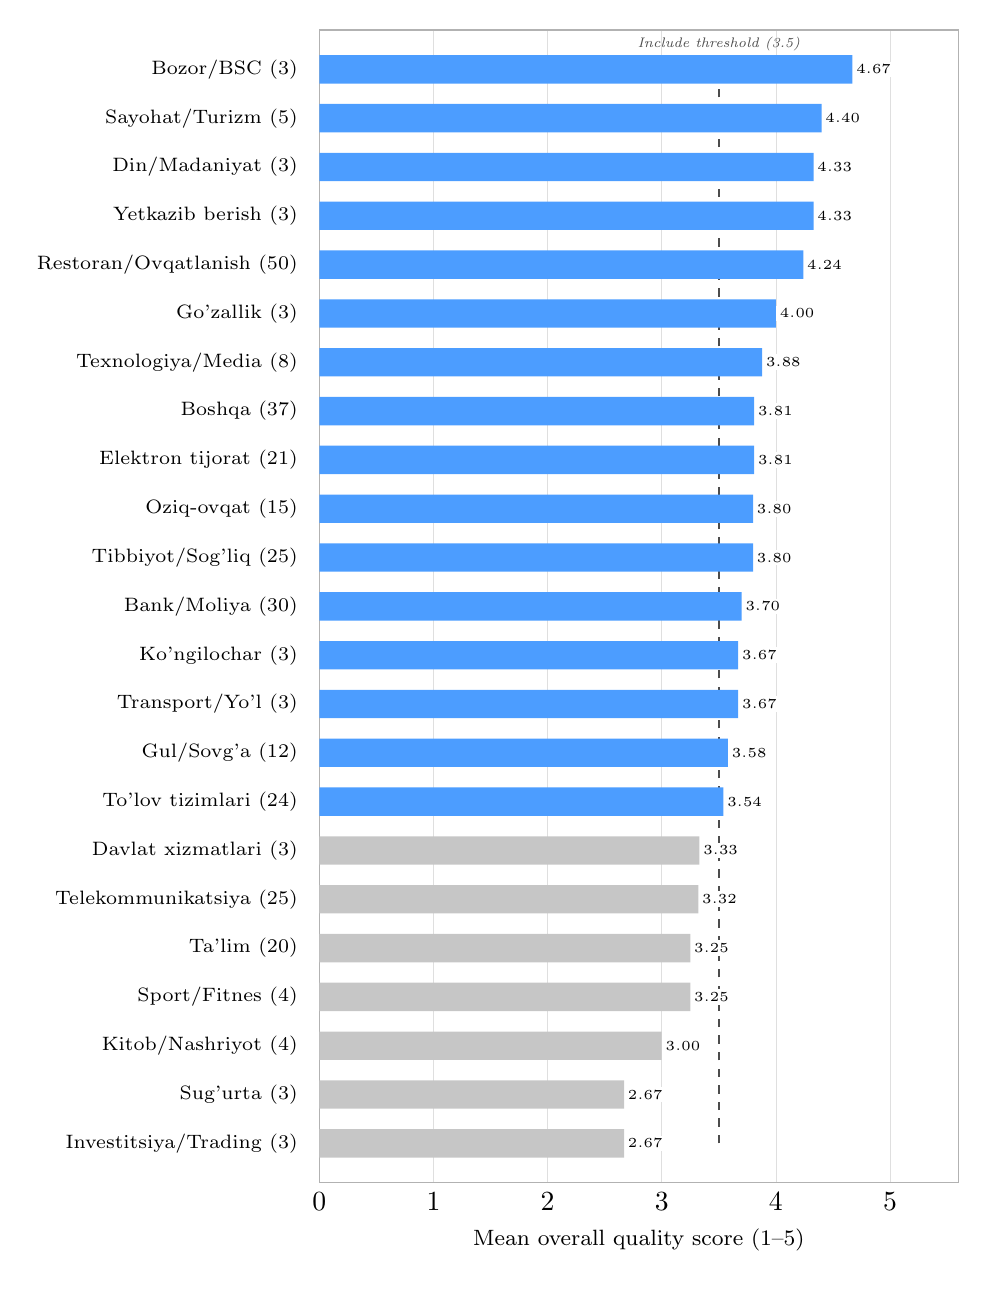
\begin{tikzpicture}
\begin{axis}[
  xbar,
  width=0.8\textwidth,
  xmin=0, xmax=5.6,
  xlabel={Mean overall quality score (1--5)},
  xlabel style={font=\footnotesize},
  symbolic y coords={
    {Investitsiya/Trading (3)},
    {Sug'urta (3)},
    {Kitob/Nashriyot (4)},
    {Sport/Fitnes (4)},
    {Ta'lim (20)},
    {Telekommunikatsiya (25)},
    {Davlat xizmatlari (3)},
    {To'lov tizimlari (24)},
    {Gul/Sovg'a (12)},
    {Transport/Yo'l (3)},
    {Ko'ngilochar (3)},
    {Bank/Moliya (30)},
    {Tibbiyot/Sog'liq (25)},
    {Oziq-ovqat (15)},
    {Elektron tijorat (21)},
    {Boshqa (37)},
    {Texnologiya/Media (8)},
    {Go'zallik (3)},
    {Restoran/Ovqatlanish (50)},
    {Yetkazib berish (3)},
    {Din/Madaniyat (3)},
    {Sayohat/Turizm (5)},
    {Bozor/BSC (3)}
  },
  ytick={
    {Investitsiya/Trading (3)},
    {Sug'urta (3)},
    {Kitob/Nashriyot (4)},
    {Sport/Fitnes (4)},
    {Ta'lim (20)},
    {Telekommunikatsiya (25)},
    {Davlat xizmatlari (3)},
    {To'lov tizimlari (24)},
    {Gul/Sovg'a (12)},
    {Transport/Yo'l (3)},
    {Ko'ngilochar (3)},
    {Bank/Moliya (30)},
    {Tibbiyot/Sog'liq (25)},
    {Oziq-ovqat (15)},
    {Elektron tijorat (21)},
    {Boshqa (37)},
    {Texnologiya/Media (8)},
    {Go'zallik (3)},
    {Restoran/Ovqatlanish (50)},
    {Yetkazib berish (3)},
    {Din/Madaniyat (3)},
    {Sayohat/Turizm (5)},
    {Bozor/BSC (3)}
  },
  yticklabel style={font=\scriptsize},
  y=0.62cm,
  bar width=0.36cm,
  enlarge y limits={abs=0.5cm},
  axis line style={draw=gray!60},
  xmajorgrids,
  grid style={gray!25, very thin},
  tick style={draw=none},
  nodes near coords,
  % fill=white gives each value label a halo so the dashed threshold line does
  % not run through the digits of the domains sitting just below 3.5.
  nodes near coords style={font=\tiny, color=black, fill=white, inner sep=1.2pt,
    /pgf/number format/fixed, /pgf/number format/precision=2, /pgf/number format/fixed zerofill},
  clip=false,
]
% Inclusion threshold, drawn FIRST so the bars and their value labels sit on
% top of it (otherwise the dashes cut through the labels of the ~3.3 domains).
\draw[dashed, thick, black!70]
  (axis cs:3.5,{Investitsiya/Trading (3)}) -- (axis cs:3.5,{Bozor/BSC (3)})
  node[pos=1, anchor=south, yshift=3pt, font=\tiny\itshape, align=center]
    {Include threshold (3.5)};
% Domains at or above the inclusion threshold.
% bar shift=0pt: each domain appears in exactly one of the two series, so the
% default grouped-bar offset must be suppressed or every bar is drawn half a
% bar width off its own tick (and the two series collide at the threshold).
\addplot[xbar, bar shift=0pt, fill=blue!55!cyan!70, draw=none] coordinates {
  (3.54,{To'lov tizimlari (24)})
  (3.58,{Gul/Sovg'a (12)})
  (3.67,{Transport/Yo'l (3)})
  (3.67,{Ko'ngilochar (3)})
  (3.70,{Bank/Moliya (30)})
  (3.80,{Tibbiyot/Sog'liq (25)})
  (3.80,{Oziq-ovqat (15)})
  (3.81,{Elektron tijorat (21)})
  (3.81,{Boshqa (37)})
  (3.88,{Texnologiya/Media (8)})
  (4.00,{Go'zallik (3)})
  (4.24,{Restoran/Ovqatlanish (50)})
  (4.33,{Yetkazib berish (3)})
  (4.33,{Din/Madaniyat (3)})
  (4.40,{Sayohat/Turizm (5)})
  (4.67,{Bozor/BSC (3)})
};
% Domains below the inclusion threshold
\addplot[xbar, bar shift=0pt, fill=gray!45, draw=none] coordinates {
  (2.67,{Investitsiya/Trading (3)})
  (2.67,{Sug'urta (3)})
  (3.00,{Kitob/Nashriyot (4)})
  (3.25,{Sport/Fitnes (4)})
  (3.25,{Ta'lim (20)})
  (3.32,{Telekommunikatsiya (25)})
  (3.33,{Davlat xizmatlari (3)})
};
\end{axis}
\end{tikzpicture}
\caption{Mean LLM-as-Judge overall quality score for all 23 business domains (review counts in parentheses), sorted by score. Blue bars meet the inclusion threshold of 3.5 (dashed line); gray bars fall below it. The gradient runs from in-domain (\emph{Restoran/Ovqatlanish}) and vocabulary-adjacent domains at the top to specialised financial domains (\emph{Sug'urta}, \emph{Investitsiya}) at the bottom.}
\label{fig:domain_quality}
\end{figure}

\textbf{Annotation Pipeline Output.} Batch annotation of the full 5{,}038-review corpus produces 9{,}884 aspects (average 1.96 per review) with a 100\% JSON parse rate across all 23~domains. The polarity distribution is 75.1\% positive, 16.5\% negative, and 8.4\% neutral---reflecting a natural skew in user-generated reviews. The aspect category distribution reveals a notable pattern: \emph{boshqalar} (miscellaneous) dominates at 45.5\%, followed by \emph{ovqat} (17.9\%), \emph{xizmat} (15.9\%), \emph{muhit} (10.7\%), and \emph{narx} (9.0\%).

% ----------------------------------------------------------------------
\subsection{Human Validation of Annotation Quality}
\label{sec:res_human}

Because both the silver annotations and their quality scores originate from models, we validate a subsample against native-speaker judgement. Two native Uzbek speakers---the second and third authors---annotated a stratified subsample of 150 reviews drawn from the 307 judged reviews (all 23 domains represented, deliberately oversampling distant and low-scoring domains), performing two tasks: (i) rating the model's predicted annotations on the same five-dimension 1--5 rubric used by the LLM judge, and (ii) re-annotating a subset of 80 reviews from scratch to obtain human gold references.

\textbf{Inter-annotator agreement.} Rubric ratings were produced after a joint calibration pass on the 1--5 scale. \Cref{tab:iaa} reports agreement between the two raters on all 150 reviews, measured with quadratic-weighted Cohen's $\kappa$ (which penalises large rating gaps more than adjacent ones) and Krippendorff's $\alpha$ on the interval scale. Agreement is high and consistent across dimensions ($\kappa = 0.911$--$0.970$, $\alpha = 0.911$--$0.970$), highest on sentiment correctness ($\kappa = 0.970$) and lowest on relevance ($\kappa = 0.911$); Spearman correlations between raters fall in the same band ($\rho = 0.920$--$0.941$). The two raters therefore apply the rubric consistently enough for their mean rating to serve as the reference against which the LLM judge is calibrated below.

\begin{table}[t]
\centering
\caption{Inter-annotator agreement between the two native-speaker raters on the 150-review rubric sample, per dimension. $\kappa$: quadratic-weighted Cohen's kappa; $\alpha$: Krippendorff's alpha (interval); $\rho$: Spearman rank correlation.}
\label{tab:iaa}
\begin{tabular}{lccc}
\toprule
\textbf{Dimension} & \textbf{Weighted $\kappa$} & \textbf{Krippendorff's $\alpha$} & \textbf{Spearman $\rho$} \\
\midrule
Sentiment    & 0.970 & 0.970 & 0.941 \\
Accuracy     & 0.936 & 0.936 & 0.920 \\
Completeness & 0.930 & 0.930 & 0.937 \\
Overall      & 0.923 & 0.922 & 0.923 \\
Relevance    & 0.911 & 0.911 & 0.925 \\
\bottomrule
\end{tabular}
\end{table}

Gold annotation followed a two-stage protocol. In the first, fully independent pass, the two annotators' span-level agreement was low (exact-match F1 0.277, partial 0.415)---not because they disagreed about opinions, but because their segmentation and normalization conventions diverged (lemmatized vs.\ surface forms; naming the referent rather than the mention); polarity agreement on matched terms was perfect. In the second stage the annotators reconciled conventions and produced a consolidated reference with high residual span agreement (exact F1 0.927, polarity 100\%), released as the reconciled double-annotated subset (\texttt{gold80}) alongside the silver corpus; because the reconciliation involved the same two annotators, we refrain from calling it fully adjudicated gold until an independent third annotator has resolved the residual disagreements. This two-stage outcome is itself informative: even for native speakers, \emph{what counts as the aspect span} is the dominant source of ABSA annotation disagreement in Uzbek, while polarity is essentially unambiguous.

\textbf{Judge calibration.} \Cref{tab:judge_calibration} compares GPT-4o-mini's scores with the mean human rating on the same 150 reviews. Rank correlations are moderate to strong on the dimensions that drive dataset assembly---sentiment ($\rho=0.81$), relevance ($\rho=0.67$), and the tier-defining overall score ($\rho=0.66$; all $p<10^{-6}$)---and the judge's mean overall score (3.75) closely matches the human mean (3.84). Correlations are weaker for completeness and accuracy ($\rho\approx0.43$--0.46), where the judge is systematically harsher on completeness (mean 3.30 vs.\ 4.04). We conclude that the LLM judge is a usable, though imperfect, proxy for native-speaker quality judgement, and that its quality tiers rank annotations in an order humans broadly agree with.

\begin{table}[t]
\centering
\caption{Calibration of the GPT-4o-mini judge against the mean rating of two native-speaker annotators on the same 150 reviews (Spearman $\rho$, all $p<10^{-6}$; MAE on the 1--5 scale).}
\label{tab:judge_calibration}
\begin{tabular}{lcccc}
\toprule
\textbf{Dimension} & \textbf{$\rho$} & \textbf{MAE} & \textbf{Human mean} & \textbf{Judge mean} \\
\midrule
Sentiment    & 0.806 & 0.34 & 4.25 & 4.24 \\
Relevance    & 0.667 & 0.50 & 3.85 & 3.97 \\
Overall      & 0.657 & 0.55 & 3.84 & 3.75 \\
Accuracy     & 0.433 & 0.54 & 4.19 & 4.44 \\
Completeness & 0.462 & 0.94 & 4.04 & 3.30 \\
\bottomrule
\end{tabular}
\end{table}

\textbf{Model vs.\ human gold.} Against the consolidated gold references, the model achieves exact-match ATE F1 of 0.209--0.224 and partial-match F1 of 0.425--0.433 (per annotator), with 100\% polarity agreement on exactly matched terms. Two reference points contextualize these scores. First, the model's partial-match agreement ($\approx$0.43) matches the level two humans reach \emph{before} convention reconciliation (0.415), while falling well short of the reconciled ceiling (0.93)---the gap is concentrated in span segmentation, not in opinion detection or polarity. Second, across domain-proximity groups the human-measured quality reproduces the judge's gradient, falling from 0.244 exact pair F1 on general out-of-domain reviews to 0.170 on the most distant domains. We note the scope of this study: both annotators are authors of this paper, so the validation is internal rather than independent, and the sample sizes per domain are small; a larger validation with fully external annotators is left for future work.


%%%%%%%%%%%%%%%%%%%%%%%%%%%%%%%%%%%%%%%%%%

\section{Discussion}
\label{sec:discussion}

% ----------------------------------------------------------------------
\textbf{The Completeness Bottleneck}. Completeness (mean 3.32/5) is the worst quality dimension: the model successfully captures characteristics that are present in the text but sometimes misses domain-specific or subtle viewpoints, especially outside the restaurant domain. This is mainly due to the poor coverage of the training data, only five aspect categories, and the model has to map the unseen aspects to the generic \textit{boshqalar} (miscellaneous) label, which is predominant with 45.5\%. To solve this bottleneck, we would have to undertake domain-adaptive fine-tuning or expand the aspect taxonomy to better capture out-of-domain phenomena.

% ----------------------------------------------------------------------
\textbf{Checkpoint Effects}. R1 reasoning distillation conferred no advantage on structured ABSA in this setting: despite sharing the Qwen-7B backbone, the distilled checkpoint underperformed both Qwen and Llama. The zero-shot controls isolate part of the mechanism directly: unadapted, the R1 checkpoint's reasoning traces break JSON parsing on more than half the evaluation examples (\Cref{tab:zeroshot}), so reasoning-oriented output habits demonstrably sit awkwardly against strict formatting---and even after fine-tuning suppresses the preamble, no residual benefit appears. Llama achieves the lowest loss and best sentiment accuracy, but Qwen is superior for reliable extraction and instruction following (100\% parse rate, highest ATE recall). For annotation pipelines, robust JSON compliance and extraction coverage are more critical than marginal gains in sentiment metrics.

% ----------------------------------------------------------------------
\textbf{Is a 7B LLM Worth It?} The practical image is clearer with the encoder baselines. We observe no statistically significant difference from the 7–8B LLMs for aspect-term extraction with a 110M monolingual encoder fine-tuned in ten minutes on a laptop, a reminder that for span identification in a morphologically rich language targeted monolingual pre-training (BERTbek, TahrirchiBERT) remains remarkably effective. The LLMs justify their cost where the task is truly joint and generative: sentiment macro-F1 (+5--7 points over the encoders), unified term- and category-level output in a single generation, and the ability to follow natural-language instructions on unseen domains, which is what the multi-domain annotation pipeline exploits. Therefore, teams designing Uzbek ABSA systems under constrained computational constraints should consider encoders for extraction-only workloads and reserve LLMs for simultaneous prediction and annotation-generation scenarios.

% ----------------------------------------------------------------------
\textbf{Loss as a Model Selection Proxy}. Validation loss ranking diverges from ABSA performance: Llama's lowest loss does not translate to the best extraction, while Qwen outperforms on ATE F1 despite higher loss. Cross-entropy loss captures token-level likelihood but not structured-output quality such as JSON validity or aspect-boundary precision. This divergence is expected for structured-generation tasks, yet it is easy to overlook in practice; model selection for ABSA is therefore better guided by task-specific metrics than by validation loss alone.

% ----------------------------------------------------------------------
\textbf{Limitations}. This study trains exclusively on restaurant reviews, without domain-adaptive fine-tuning; cross-domain performance should therefore be read as a demonstration of pipeline feasibility rather than a claim of uniform quality, and indeed we observe measurable degradation on distant domains. While we validate a stratified subset of the multi-domain corpus against native-speaker annotations (\Cref{sec:res_human}), the released dataset remains predominantly silver-standard: the human-verified portion is an 80-review subset produced by two native-speaker annotators under a two-stage reconciliation protocol, and the remaining annotations carry only model- and judge-derived quality estimates. Positive polarity dominates both datasets, and compute constraints meant the model comparison reuses the fixed evaluation split rather than a separately retrained held-out test set; for the same reason, statistical significance testing covers the encoder pair, while the LLM--encoder gaps are reported descriptively.

Several evaluation-design caveats remain. First, the 609-example split functions as a development set: evaluation loss on it is monitored during training (every 100 steps), and the same partition is then reused for the headline numbers, so the reported scores are optimistic relative to a genuinely untouched test set; a three-way train/development/test partition is the main methodological upgrade we would make with a larger corpus. Second, although the split is deduplicated by review text (\Cref{sec:res_split}) and now controlled against zero-shot baselines (\Cref{sec:res_zeroshot}), robustness to random seeds is only partially characterized: a single replicate (for Qwen) bounds seed variation at roughly $\pm 0.01$ F1, but multi-seed replication of every system---which \Cref{tab:split_effect} suggests matters at exactly the scale of the observed inter-model gaps---remains undone. Third, few-shot prompting sits unexplored between the zero-shot controls and full fine-tuning, so we cannot say how much of the QLoRA gain cheaper in-context adaptation could recover. Finally, the multi-domain case study (\Cref{sec:res_multidomain}) was produced with the annotation engine fine-tuned under the earlier revision of the preprocessing pipeline; since its output quality is assessed directly---by the LLM judge and the native-speaker validation study---the case-study conclusions are unaffected, but the released silver annotations do not benefit from the improvements in \Cref{tab:split_effect}, and regenerating them with the corrected model is planned for the next dataset version. Tokenizer efficiency and larger-scale, convention-reconciled human verification remain for future work.

%%%%%%%%%%%%%%%%%%%%%%%%%%%%%%%%%%%%%%%%%%


%%%%%%%%%%%%%%%%%%%%%%%%%%%%%%%%%%%%%%%%%%
\section{Conclusions}
\label{sec:conclusion}
This paper presented is the first systematic study of parameter-efficient fine-tuning of open-weight LLMs for Uzbek ABSA. We showed that QLoRA enables effective joint aspect extraction and sentiment classification via structured JSON generation---at least doubling extraction F1 and tripling end-to-end pair F1 over unadapted zero-shot controls---and that the fine-tuned LLMs are competitive with fine-tuned Uzbek BERT encoders. Our comparison revealed a clear architectural trade-off: Qwen~2.5-7B excels at reliable aspect extraction and instruction following, whereas Llama~3.1-8B achieves the highest precision for end-to-end sentiment matching, with the two effectively tied on end-to-end F1. We also found that validation loss is an unreliable proxy for downstream structured-extraction performance. Finally, we showed that a model trained only on restaurant reviews can produce usable annotations on more distant domains, though quality degrades measurably with domain distance. Our three-layer pipeline, together with a human-validation study of its output, produced a quality-scored multi-domain silver-standard resource with a gold-verified subset, offering a practical route to scalable low-resource dataset creation. Future work will focus on expanding the aspect taxonomy, on domain-adaptive fine-tuning to increase completeness of extraction across different business domains, and on injecting the morphosyntactic structure now available from Uzbek Universal Dependencies treebanks and parsers \cite{MATLATIPOV2026112857,11632281,10.1007/978-3-032-29532-3_15} into the extraction step since span segmentation, not opinion detection, is where both our models and human annotators disagreed the most (\Cref{sec:res_human}).
%%%%%%%%%%%%%%%%%%%%%%%%%%%%%%%%%%%%%%%%%%
\vspace{6pt} 

%%%%%%%%%%%%%%%%%%%%%%%%%%%%%%%%%%%%%%%%%%
%% optional
%\supplementary{The following supporting information can be downloaded at:  \linksupplementary{s1}, Figure S1: title; Table S1: title; Video S1: title.}

% Only for journal Methods and Protocols:
% If you wish to submit a video article, please do so with any other supplementary material.
% \supplementary{The following supporting information can be downloaded at: \linksupplementary{s1}, Figure S1: title; Table S1: title; Video S1: title. A supporting video article is available at doi: link.}

% Only used for preprtints:
% \supplementary{The following supporting information can be downloaded at the website of this paper posted on \href{https://www.preprints.org/}{Preprints.org}.}

% Only for journal Hardware:
% If you wish to submit a video article, please do so with any other supplementary material.
% \supplementary{The following supporting information can be downloaded at: \linksupplementary{s1}, Figure S1: title; Table S1: title; Video S1: title.\vspace{6pt}\\
%\begin{tabularx}{\textwidth}{lll}
%\toprule
%\textbf{Name} & \textbf{Type} & \textbf{Description} \\
%\midrule
%S1 & Python script (.py) & Script of python source code used in XX \\
%S2 & Text (.txt) & Script of modelling code used to make Figure X \\
%S3 & Text (.txt) & Raw data from experiment X \\
%S4 & Video (.mp4) & Video demonstrating the hardware in use \\
%... & ... & ... \\
%\bottomrule
%\end{tabularx}
%}

%%%%%%%%%%%%%%%%%%%%%%%%%%%%%%%%%%%%%%%%%%
\authorcontributions{Conceptualization, S.M. and M.A.; methodology, S.M. and M.A.; software, S.M.; validation, S.M. and J.R.; formal analysis, S.M. and A.M.A.; investigation, S.M. and J.R.; resources, M.A.; data curation, S.M. and J.R.; writing---original draft preparation, S.M.; writing---review and editing, S.M., M.A., J.R. and A.M.A.; visualization, S.M.; supervision, M.A.; project administration, S.M.; funding acquisition, not applicable. All authors have read and agreed to the published version of the manuscript.}

\funding{This research received no external funding.}

\institutionalreview{Not applicable.}

\informedconsent{Not applicable. The study analyses publicly accessible user-generated business reviews and does not involve direct interaction with human participants. The reviews were used with explicit permission from the platform owner (see \Cref{sec:acknowledgement}).}

\dataavailability{The primary Uzbek aspect-based sentiment analysis dataset used for model fine-tuning is publicly available on Hugging Face at \url{https://huggingface.co/datasets/Sanatbek/aspect-based-sentiment-analysis-uzbek}. The multi-domain Uzbek business review corpus generated in this study, including the 80-review reconciled double-annotated subset (\Cref{sec:res_human}), is publicly available on Zenodo at \url{https://zenodo.org/records/22146677} with DOI: \href{https://doi.org/10.5281/zenodo.22146677}{10.5281/zenodo.22146677}. The released records contain the review text, business category and name, the star rating, and the annotation and quality metadata; contributor user names, review URLs, and posting timestamps present in the source platform are deliberately excluded. Code for the encoder baselines, the human-validation analysis, and the significance tests is available in the project repository.
}

%\durcstatement{Current research is limited to the [please insert a specific academic field, e.g., XXX], which is beneficial [share benefits and/or primary use] and does not pose a threat to public health or national security. Authors acknowledge the dual-use potential of the research involving xxx and confirm that all necessary precautions have been taken to prevent potential misuse. As an ethical responsibility, authors strictly adhere to relevant national and international laws about DURC. Authors advocate for responsible deployment, ethical considerations, regulatory compliance, and transparent reporting to mitigate misuse risks and foster beneficial outcomes.}

% Only for journal Nursing Reports
%\publicinvolvement{Please describe how the public (patients, consumers, carers) were involved in the research. Consider reporting against the GRIPP2 (Guidance for Reporting Involvement of Patients and the Public) checklist. If the public were not involved in any aspect of the research add: ``No public involvement in any aspect of this research''.}
%
%% Only for journal Nursing Reports
%\guidelinesstandards{Please add a statement indicating which reporting guideline was used when drafting the report. For example, ``This manuscript was drafted against the XXX (the full name of reporting guidelines and citation) for XXX (type of research) research''. A complete list of reporting guidelines can be accessed via the equator network: \url{https://www.equator-network.org/}.}
%
%% Only for journal Nursing Reports
%\useofartificialintelligence{Please describe in detail any and all uses of artificial intelligence (AI) or AI-assisted tools used in the preparation of the manuscript. This may include, but is not limited to, language translation, language editing and grammar, or generating text. Alternatively, please state that “AI or AI-assisted tools were not used in drafting any aspect of this manuscript”.}

\acknowledgments{\label{sec:acknowledgement}We extend our heartfelt gratitude to Sardor Berdiyev, CEO and Co-founder of Commeta, for graciously granting permission to use publicly available reviews from the sharh.commeta.uz platform exclusively for academic research purposes. We also acknowledge the computational resources provided by the National University of Uzbekistan. During the preparation of this manuscript/study, the authors used Anthropic Claude (Sonnet~5 and Opus~5) for the purposes of paraphrasing, language editing, and manuscript revision. The authors have reviewed and edited the output and take full responsibility for the content of this publication.}


\conflictsofinterest{ The authors declare no conflicts of interest.} 

%%%%%%%%%%%%%%%%%%%%%%%%%%%%%%%%%%%%%%%%%%
%% Optional

%% Only for journal Encyclopedia
%\entrylink{The Link to this entry published on the encyclopedia platform.}

\abbreviations{Abbreviations}{
The following abbreviations are used in this manuscript:
\\

\noindent 
\begin{tabular}{@{}ll}
ABSA & Aspect-Based Sentiment Analysis\\
ACD & Aspect Category Detection\\
ASC & Aspect Sentiment Classification\\
ATE & Aspect Term Extraction\\
QLoRA & Quantized Low-Rank Adaptation
\end{tabular}
}

%%%%%%%%%%%%%%%%%%%%%%%%%%%%%%%%%%%%%%%%%%
\appendixtitles{yes}
\appendixstart
\appendix
\section[\appendixname~\thesection]{Full Per-Domain LLM-as-Judge Quality Scores}
\label{sec:appendix_domains}

\Cref{tab:domain_quality_full} reports LLM-as-Judge quality scores for all 23 business domains in the stratified evaluation sample (307 reviews total). The main text (\Cref{tab:domain_quality}) presents a selected subset grouped by training-distribution proximity; this table provides the complete picture, sorted by overall quality score in descending order. Scores are on a 1--5 Likert scale across five dimensions: Completeness, Accuracy (hallucination control), Sentiment Correctness, Relevance (category--domain fit), and Overall. Domains with $N \leq 5$ should be interpreted with caution due to small sample sizes. The ``Include'' threshold (Overall $\geq 3.5$) is shown as a dashed reference.

\begin{table}[H]
\centering
\caption{LLM-as-Judge (GPT-4o-mini) quality scores for all 23 business domains, sorted by Overall score (descending). Stratified evaluation sample: 307 reviews. Scale: 1--5 (higher is better). $^{*}$~Small sample ($N \leq 5$): interpret with caution.\label{tab:domain_quality_full}}
\setlength{\tabcolsep}{3.5pt}
\small
\begin{tabular}{llccccc}
\toprule
\textbf{Domain (Uzbek / English)} & $N$ & \textbf{Comp.} & \textbf{Acc.} & \textbf{Sent.} & \textbf{Rel.} & \textbf{Overall} \\
\midrule
Bozor/BSC (Market/Shopping centre)$^{*}$ & 3  & 3.67 & 5.00 & 5.00 & 5.00 & 4.67 \\
Sayohat/Turizm (Tourism/Travel)$^{*}$   & 5  & 4.00 & 4.80 & 4.60 & 4.40 & 4.40 \\
Din/Madaniyat (Religion/Culture)$^{*}$   & 3  & 4.33 & 5.00 & 4.00 & 5.00 & 4.33 \\
Yetkazib berish (Delivery)$^{*}$          & 3  & 3.67 & 5.00 & 4.67 & 4.33 & 4.33 \\
Restoran/Ovqatlanish (Restaurant/Dining)      & 50 & 3.68 & 4.76 & 4.56 & 4.66 & 4.24 \\
Go'zallik (Beauty services)$^{*}$         & 3  & 3.33 & 4.67 & 5.00 & 4.00 & 4.00 \\
Texnologiya/Media (Technology/Media)          & 8  & 2.88 & 4.50 & 5.00 & 3.88 & 3.88 \\
Boshqa (Other/Miscellaneous)                  & 37 & 3.43 & 4.54 & 3.89 & 4.38 & 3.81 \\
Elektron tijorat (E-commerce)                 & 21 & 3.43 & 4.48 & 4.10 & 4.14 & 3.81 \\
Oziq-ovqat do'konlari (Grocery stores)        & 15 & 3.47 & 4.33 & 4.47 & 4.13 & 3.80 \\
Tibbiyot/Sog'liqni saqlash (Healthcare)       & 25 & 3.40 & 4.60 & 4.20 & 4.36 & 3.80 \\
Bank/Moliya (Banking/Finance)                 & 30 & 3.40 & 4.47 & 4.17 & 3.90 & 3.70 \\
Ko'ngilochar (Entertainment)$^{*}$        & 3  & 3.33 & 4.67 & 4.33 & 4.00 & 3.67 \\
Transport/Yo'l (Transport/Roads)$^{*}$    & 3  & 3.33 & 4.00 & 4.00 & 4.00 & 3.67 \\
Gul/Sovg'a (Flowers/Gifts)                    & 12 & 3.08 & 4.08 & 4.83 & 3.67 & 3.58 \\
To'lov tizimlari (Payment systems)            & 24 & 3.00 & 4.29 & 4.38 & 3.54 & 3.54 \\
\midrule
\multicolumn{7}{l}{\textit{Below inclusion threshold (Overall $< 3.5$)}} \\
\midrule
Davlat xizmatlari (Government services)$^{*}$ & 3 & 3.00 & 4.00 & 4.33 & 3.67 & 3.33 \\
Telekommunikatsiya (Telecommunications)       & 25 & 3.04 & 4.36 & 3.64 & 3.64 & 3.32 \\
Ta'lim (Education)                            & 20 & 2.90 & 4.20 & 3.80 & 3.45 & 3.25 \\
Sport/Fitnes (Gyms/Fitness)$^{*}$          & 4  & 2.75 & 4.25 & 4.25 & 3.00 & 3.25 \\
Kitob/Nashriyot (Books/Publishing)$^{*}$  & 4  & 3.00 & 4.25 & 4.00 & 3.00 & 3.00 \\
Sug'urta (Insurance)$^{*}$                & 3  & 2.33 & 3.67 & 2.67 & 3.33 & 2.67 \\
Investitsiya/Trading (Investment)$^{*}$   & 3  & 2.33 & 4.00 & 3.67 & 3.00 & 2.67 \\
\bottomrule
\end{tabular}
\end{table}

\section[\appendixname~\thesection]{Bootstrap Confidence Intervals for All Systems}
\label{sec:appendix_cis}

\Cref{tab:cis} reports exact percentile-bootstrap 95\% confidence intervals ($B{=}10{,}000$ resamples over the 609 evaluation reviews) for every score in \Cref{tab:absa_results}. Half-widths range from $\pm 0.023$ (Llama sentiment accuracy) to $\pm 0.037$ (DeepSeek pair F1), and the intervals of the top-ranked systems overlap substantially on all four metrics---the reason the paired-bootstrap comparisons in \Cref{sec:res_comparison} detect so few significant differences. Note that these are per-system intervals on absolute scores; because the systems are evaluated on identical reviews, the \emph{paired} tests in \Cref{sec:res_comparison} are more powerful than a visual comparison of these intervals would suggest.

\begin{table}[H]
\centering
\caption{Percentile-bootstrap 95\% confidence intervals ($B{=}10{,}000$, resampling reviews) for each system on the 609-example evaluation set. Estimates match \Cref{tab:absa_results}.\label{tab:cis}}
\setlength{\tabcolsep}{3pt}
\footnotesize
\begin{tabular}{lcccc}
\toprule
\textbf{System} & \textbf{ATE exact F1} & \textbf{ATE partial F1} & \textbf{Pair F1} & \textbf{Sent. Acc.} \\
\midrule
\multicolumn{5}{l}{\textit{QLoRA fine-tuned LLMs}} \\
Qwen 2.5-7B      & 0.708 [0.674, 0.740] & 0.802 [0.775, 0.829] & 0.645 [0.608, 0.680] & 0.911 [0.886, 0.935] \\
Llama 3.1-8B     & 0.704 [0.670, 0.737] & 0.801 [0.773, 0.828] & 0.651 [0.615, 0.687] & 0.925 [0.901, 0.947] \\
DeepSeek-R1-7B   & 0.678 [0.642, 0.714] & 0.787 [0.758, 0.817] & 0.603 [0.566, 0.640] & 0.891 [0.860, 0.918] \\
\midrule
\multicolumn{5}{l}{\textit{Fine-tuned Uzbek encoders}} \\
BERTbek          & 0.692 [0.657, 0.726] & 0.800 [0.774, 0.826] & 0.608 [0.571, 0.644] & 0.879 [0.851, 0.906] \\
TahrirchiBERT    & 0.701 [0.667, 0.734] & 0.787 [0.758, 0.814] & 0.623 [0.586, 0.657] & 0.889 [0.862, 0.915] \\
\bottomrule
\end{tabular}
\end{table}

%%%%%%%%%%%%%%%%%%%%%%%%%%%%%%%%%%%%%%%%%%
%\isPreprints{}{% This command is only used for ``preprints''.
\begin{adjustwidth}{-\extralength}{0cm}
%} % If the paper is ``preprints'', please uncomment this parenthesis.
%\printendnotes[custom] % Un-comment to print a list of endnotes

\reftitle{References}

% Please provide either the correct journal abbreviation (e.g. according to the “List of Title Word Abbreviations” http://www.issn.org/services/online-services/access-to-the-ltwa/) or the full name of the journal.
% Citations and References in Supplementary files are permitted provided that they also appear in the reference list here. 

%=====================================
% References, variant A: external bibliography
%=====================================
\bibliography{mybibliography}

%=====================================
% References, variant B: internal bibliography
%=====================================

% ACS format
% \isAPAandChicago{}{%
% \begin{thebibliography}{999}
% % Reference 1
% \bibitem[Author1(year)]{ref-journal}
% Author~1, T. The title of the cited article. {\em Journal Abbreviation} {\bf 2008}, {\em 10}, 142--149.
% % Reference 2
% \bibitem[Author2(year)]{ref-book1}
% Author~2, L. The title of the cited contribution. In {\em The Book Title}; Editor 1, F., Editor 2, A., Eds.; Publishing House: City, Country, 2007; pp. 32--58.
% % Reference 3
% \bibitem[Author1 and Author2 (year)]{ref-book2}
% Author 1, A.; Author 2, B. \textit{Book Title}, 3rd ed.; Publisher: Publisher Location, Country, 2008; pp. 154--196.
% % Reference 4
% \bibitem[Author4(year)]{ref-unpublish}
% Author 1, A.B.; Author 2, C. Title of Unpublished Work. \textit{Abbreviated Journal Name} year, \textit{phrase indicating stage of publication (submitted; accepted; in press)}.
% % Reference 5
% \bibitem[Author8(year)]{ref-url}
% Title of Site. Available online: URL (accessed on Day Month Year).
% % Reference 6
% \bibitem[Author6(year)]{ref-proceeding}
% Author 1, A.B.; Author 2, C.D.; Author 3, E.F. Title of presentation. In Proceedings of the Name of the Conference, Location of Conference, Country, Date of Conference (Day Month Year); Abstract Number (optional), Pagination (optional).
% % Reference 7
% \bibitem[Author7(year)]{ref-thesis}
% Author 1, A.B. Title of Thesis. Level of Thesis, Degree-Granting University, Location of University, Date of Completion.
% \end{thebibliography}
% }

% % Chicago format (Used for journal: arts, genealogy, histories, humanities, jintelligence, laws, literature, religions, risks, socsci)
% \isChicagoStyle{%
% \begin{thebibliography}{999}
% % Reference 1
% \bibitem[Aranceta-Bartrina(1999a)]{ref-journal}
% Aranceta-Bartrina, Javier. 1999a. Title of the cited article. \textit{Journal Title} 6: 100--10.
% % Reference 2
% \bibitem[Aranceta-Bartrina(1999b)]{ref-book1}
% Aranceta-Bartrina, Javier. 1999b. Title of the chapter. In \textit{Book Title}, 2nd ed. Edited by Editor 1 and Editor 2. Publication place: Publisher, vol. 3, pp. 54–96.
% % Reference 3
% \bibitem[Baranwal and Munteanu {[1921]}(1955)]{ref-book2}
% Baranwal, Ajay K., and Costea Munteanu. 1955. \textit{Book Title}. Publication place: Publisher, pp. 154--96. First published 1921 (op-tional).
% % Reference 4
% \bibitem[Berry and Smith(1999)]{ref-thesis}
% Berry, Evan, and Amy M. Smith. 1999. Title of Thesis. Level of Thesis, Degree-Granting University, City, Country. Identifi-cation information (if available).
% % Reference 5
% \bibitem[Cojocaru et al.(1999)]{ref-unpublish}
% Cojocaru, Ludmila, Dragos Constatin Sanda, and Eun Kyeong Yun. 1999. Title of Unpublished Work. \textit{Journal Title}, phrase indicating stage of publication.
% % Reference 6
% \bibitem[Driver et al.(2000)]{ref-proceeding}
% Driver, John P., Steffen Rohrs, and Sean Meighoo. 2000. Title of Presentation. In \textit{Title of the Collected Work} (if available). Paper presented at Name of the Conference, Location of Conference, Date of Conference.
% % Reference 7
% \bibitem[Harwood(2008)]{ref-url}
% Harwood, John. 2008. Title of the cited article. Available online: URL (accessed on Day Month Year).
% \end{thebibliography}
% }{}

% % APA format (Used for journal: admsci, behavsci, businesses, econometrics, economies, education, ejihpe, games, humans, ijfs, journalmedia, jrfm, languages, psycholint, publications, tourismhosp, youth)
% \isAPAStyle{%
% \begin{thebibliography}{999}
% % Reference 1
% \bibitem[\protect\citeauthoryear{Azikiwe \BBA\ Bello}{{2020a}}]{ref-journal}
% Azikiwe, H., \& Bello, A. (2020a). Title of the cited article. \textit{Journal Title}, \textit{Volume}(Issue), 
% Firstpage--Lastpage/Article Number.
% % Reference 2
% \bibitem[\protect\citeauthoryear{Azikiwe \BBA\ Bello}{{2020b}}]{ref-book1}
% Azikiwe, H., \& Bello, A. (2020b). \textit{Book title}. Publisher Name.
% % Reference 3
% \bibitem[Davison(1623/2019)]{ref-book2}
% Davison, T. E. (2019). Title of the book chapter. In A. A. Editor (Ed.), \textit{Title of the book: Subtitle} 
% (pp. Firstpage--Lastpage). Publisher Name. (Original work published 1623) (Optional).
% % Reference 4
% \bibitem[Fistek et al.(2017)]{ref-proceeding}
% Fistek, A., Jester, E., \& Sonnenberg, K. (2017, Month Day). Title of contribution [Type of contribution]. Conference Name, Conference City, Conference Country.
% % Reference 5
% \bibitem[Hutcheson(2012)]{ref-thesis}
% Hutcheson, V. H. (2012). \textit{Title of the thesis} [XX Thesis, Name of Institution Awarding the Degree].
% % Reference 6
% \bibitem[Lippincott \& Poindexter(2019)]{ref-unpublish}
% Lippincott, T., \& Poindexter, E. K. (2019). \textit{Title of the unpublished manuscript} [Unpublished manuscript/Manuscript in prepara-tion/Manuscript submitted for publication]. Department Name, Institution Name.
% % Reference 7
% \bibitem[Harwood(2008)]{ref-url}
% Harwood, J. (2008). \textit{Title of the cited article}. Available online: URL (accessed on Day Month Year).
% \end{thebibliography}
% }{}

% If authors have biography, please use the format below
%\section*{Short Biography of Authors}
%\bio
%{\raisebox{-0.35cm}{\includegraphics[width=3.5cm,height=5.3cm,clip,keepaspectratio]{Definitions/author1.pdf}}}
%{\textbf{Firstname Lastname} Biography of first author}
%
%\bio
%{\raisebox{-0.35cm}{\includegraphics[width=3.5cm,height=5.3cm,clip,keepaspectratio]{Definitions/author2.jpg}}}
%{\textbf{Firstname Lastname} Biography of second author}

% For the MDPI journals use author-date citation, please follow the formatting guidelines on http://www.mdpi.com/authors/references
% To cite two works by the same author: \citeauthor{ref-journal-1a} (\citeyear{ref-journal-1a}, \citeyear{ref-journal-1b}). This produces: Whittaker (1967, 1975)
% To cite two works by the same author with specific pages: \citeauthor{ref-journal-3a} (\citeyear{ref-journal-3a}, p. 328; \citeyear{ref-journal-3b}, p.475). This produces: Wong (1999, p. 328; 2000, p. 475)

%%%%%%%%%%%%%%%%%%%%%%%%%%%%%%%%%%%%%%%%%%
%% for journal Sci
%\reviewreports{\\
%Reviewer 1 comments and authors’ response\\
%Reviewer 2 comments and authors’ response\\
%Reviewer 3 comments and authors’ response
%}
%%%%%%%%%%%%%%%%%%%%%%%%%%%%%%%%%%%%%%%%%%
\PublishersNote{}
%\isPreprints{}{% This command is only used for ``preprints''.
\end{adjustwidth}
%} % If the paper is ``preprints'', please uncomment this parenthesis.
\end{document}

